\documentclass[conference]{IEEEtran}
\usepackage{iftex}
\ifPDFTeX
  \usepackage[utf8]{inputenc}
  \usepackage[T1]{fontenc}
\fi
\usepackage[spanish,es-tabla,es-nodecimaldot]{babel}
\unaccentedoperators
\usepackage{microtype}
\usepackage{cite}
\usepackage{amsmath,amssymb,graphicx}
\usepackage{booktabs}
\usepackage{placeins}
\usepackage{xcolor}
\usepackage[hidelinks]{hyperref}

\makeatletter
\def\@seccntformat#1{\csname the#1dis\endcsname\hskip 0.5em\relax}
\makeatother

\addto\captionsspanish{%
  \renewcommand{\tablename}{TABLA}%
  \renewcommand{\figurename}{Fig.}%
  \renewcommand{\abstractname}{Resumen}%
  \renewcommand{\refname}{\ifPDFTeX Referencias\else REFERENCIAS\fi}%
}

\ifPDFTeX
  \newcommand{\secUC}[1]{#1}
\else
  \newcommand{\secUC}[1]{\texorpdfstring{\MakeUppercase{#1}}{#1}}
\fi

\title{Cancelación de Artefactos de Movimiento en PPG: Comparación entre RLS y Variantes de LMS}

\author{%
\IEEEauthorblockN{Álvaro Martín, Elisa Fernández Morales, Thomas Michael Spitzner}
\IEEEauthorblockA{Procesamiento Adaptativo de Señales (22.46) --- Profesor: Marc S. Ressl\\
Instituto Tecnológico de Buenos Aires (ITBA), Buenos Aires, Argentina\\
Legajos: 69507, 69616, 69453 --- Email: \{almartin, efernandezmorales, tspitzner\}@itba.edu.ar}
}

\begin{document}
\maketitle

\begin{abstract}
Este informe implementa y evalúa el algoritmo \textit{Recursive Least Squares} (RLS) para cancelar artefactos de movimiento en fotopletismografía (PPG) de muñeca usando un acelerómetro triaxial como referencia, y lo compara en igualdad de condiciones con LMS, NLMS y VS-LMS sobre la base de datos IEEEPPG. Primero diagnosticamos los modos de falla del RLS convencional sobre ventanas aisladas de $8\text{ s}$ sobremuestreadas en $0.5$--$4.0\text{ Hz}$: colinealidad severa, explosión exponencial de la norma de pesos por el subespacio nulo con $\lambda<1$, sobreajuste del latido y sensibilidad a impactos impulsivos. Para resolverlos incorporamos inicialización escalada por potencia de entrada, carga diagonal persistente, recorte robusto de Huber, memoria efectiva logarítmica $N_{\text{eff}}$, precalentamiento intra-ventana y dilatación opcional de retardos ($D\in\{1,2,3,4\}$) como alternativa de condicionamiento y ahorro computacional, explorando órdenes $M\in[6,50]$. Al reoptimizar RLS, NLMS y VS-LMS sobre el mismo \textit{pipeline}, en el conjunto de prueba RLS logra el menor AAE ($11.54\text{ BPM}$ frente a $11.71$ de NLMS, $12.23$ de VS-LMS, $14.35$ de LMS y $20.41$ sin filtrar), mejor mediana ($1.30\text{ BPM}$, acorde a la literatura en ausencia de seguimiento temporal) y menos \textit{outliers} ($21.39\%$), con RMSE empatado con NLMS ($26.23$ frente a $26.22\text{ BPM}$), convergencia en frío acorde a $2L/f_s=0.38\text{ s}$ y un costo de $18.6\text{ ms}$ por ventana ($1.3\times$ NLMS). El \textit{bootstrap} por participante confirma una mejora significativa frente a no filtrar ($+8.81\text{ BPM}$) y LMS estándar ($+2.80\text{ BPM}$), pero no concluyente frente a NLMS ($+0.18\text{ BPM}$) y VS-LMS ($+0.69\text{ BPM}$) con $10$ sujetos. La ablación y el análisis modal en prueba muestran que la regularización inicial acorde a la matriz de correlación estabiliza la norma de pesos y evita errores de $23.83\text{ BPM}$ del RLS ingenuo, mientras un índice de calidad de señal (SQI) previo mejora el régimen intenso ($7.85\to 5.81\text{ BPM}$) sin aislar globalmente las fallas en reposo.
\end{abstract}

%==========================================================
\section{\secUC{Introducción}}
%==========================================================

Las señales de fotopletismografía (PPG) de muñeca permiten estimar la frecuencia cardíaca a partir de la modulación de luz verde reflejada por cambios de volumen sanguíneo. Durante el ejercicio físico intenso, los desplazamientos entre el sensor óptico y la piel inyectan artefactos de movimiento (\textit{motion artifacts}) cuya energía se superpone con la banda cardíaca ($0.5$--$4.0\text{ Hz}$), degradando la estimación de latidos por minuto (BPM)~\cite{zhang2015troika}. En la literatura de procesamiento biomédico se han abordado estas interferencias desde dos enfoques complementarios: arquitecturas con descomposición espectral y seguimiento temporal entre ventanas como TROIKA~\cite{zhang2015troika} —que reducen el error medio a $1$--$3\text{ BPM}$ mediante análisis de espectro singular y reconstrucción rala— y esquemas livianos de cancelación adaptativa de interferencia que aprovechan el acelerómetro triaxial integrado en los relojes inteligentes~\cite{wood2007lowvar,mashhadi2016hr}, frecuentemente acompañados por índices de calidad de señal (SQI) para descartar segmentos con pérdida de contacto~\cite{krishnan2010twostage,elgendi2016sqi}.

Este trabajo continúa el Proyecto~1~\cite{informe1}, donde evaluamos LMS estándar, NLMS y VS-LMS~\cite{kwong1992vslms} sobre la base de datos IEEEPPG~\cite{tan2020ieeeppg}. En aquel informe cada ventana de $8\text{ s}$ se procesó de forma independiente arrancando en frío ($\mathbf{w}[-1]=\mathbf{0}$), quedando dos limitaciones principales: la convergencia lenta de los algoritmos de gradiente frente a referencias altamente correlacionadas y la presencia de ventanas atípicas irrecuperables por impactos bruscos o pérdida de contacto óptico.

En este proyecto sustituimos los filtros de gradiente por \textit{Recursive Least Squares} (RLS)~\cite{haykin2014,ressl2026pas}, buscando una convergencia rápida e independiente de la dispersión de autovalores. Para evaluar si RLS aporta una ganancia real y a qué costo, diagnosticamos primero por qué la formulación de libro falla sobre estas ventanas, reoptimizamos NLMS y VS-LMS sobre las mismas mejoras estructurales del \textit{pipeline} para garantizar una comparación justa, verificamos la significancia estadística mediante \textit{bootstrap} por participante, cuantificamos el peso de cada componente con una ablación y sensibilidad, y evaluamos un índice de calidad de señal (SQI) previo al filtrado para descartar segmentos irrecuperables.

%==========================================================
\section{\secUC{Marco teórico}}
\label{sec:teoria}
%==========================================================

Esta sección resume el esquema heredado de~\cite{informe1} y presenta únicamente los resultados de RLS necesarios para fundamentar la implementación y las conclusiones.

\subsection{Esquema de cancelación, datos y familia LMS (resumen de~\cite{informe1})}
\label{sec:esq}

La base de datos IEEEPPG~\cite{tan2020ieeeppg} contiene registros muestreados a $f_s=125\text{ Hz}$ en ventanas de $8\text{ s}$ ($N=1000$ muestras) con paso de $2\text{ s}$ ($6\text{ s}$ de solapamiento), cada una con dos canales de PPG ($\text{PPG}_1, \text{PPG}_2$), tres ejes de aceleración ($a_x,a_y,a_z$) y el BPM de referencia obtenido de un ECG torácico. Los $22$ sujetos se dividen en entrenamiento ($12$ sujetos, $1768$ ventanas) y prueba ($10$ sujetos, $1328$ ventanas). Cada ventana se procesa de forma aislada siguiendo el \textit{pipeline} de~\cite{informe1}: filtrado pasabanda Butterworth de fase cero en $[0.5,4.0]\text{ Hz}$ ($30$--$240\text{ BPM}$), normalización por canal a media cero y varianza unitaria, armado de la matriz de regresores $\mathbf{U}\in\mathbb{R}^{N\times L}$ ($L=3M$, $M$ retardos por eje con relleno de ceros para $n<0$), filtrado adaptativo paralelo de $\text{PPG}_1$ y $\text{PPG}_2$ contra el acelerómetro, fusión lineal tardía y estimación de BPM por periodograma con \textit{zero-padding}. Para la fusión tardía se calcula el periodograma Hann de $2048$ puntos $S_k(f)$ de cada canal filtrado $e_k[n]$ ($k\in\{1,2\}$) en la banda $\mathcal{B}=[0.5,4.0]\text{ Hz}$, se localiza el pico dominante $f_{\text{pico},k}$ con vecindad $\mathcal{B}_k=\{f\in\mathcal{B}:|f-f_{\text{pico},k}|\le 0.15\text{ Hz}\}$ y se define la SNR espectral lineal en banda como
\begin{equation}
\text{SNR}_k = \frac{\sum_{f\in\mathcal{B}_k} S_k(f)}{\sum_{f\in\mathcal{B}\setminus\mathcal{B}_k} S_k(f)+\varepsilon},
\qquad w_k = \frac{\text{SNR}_k}{\text{SNR}_1+\text{SNR}_2},
\label{eq:snr_fusion}
\end{equation}
combinando ambas ramas mediante $e_{\text{fus}}[n]=w_1 e_1[n]+w_2 e_2[n]$.

En~\cite{informe1} empleamos tres variantes de gradiente estocástico de costo $\mathcal{O}(L)$ por muestra, $\mathbf{w}[n+1]=\mathbf{w}[n]+\mu_{\text{ef}}[n]\,e[n]\,\mathbf{a}[n]$, con paso efectivo $\mu_{\text{ef}}[n]=\mu$ (LMS), $\mu/(\delta_{\text{lms}}+\lVert\mathbf{a}[n]\rVert^2)$ (NLMS), y $\mu[n]/(\delta_{\text{lms}}+\lVert\mathbf{a}[n]\rVert^2)$ (VS-LMS, con $\mu[n+1]=\operatorname{clip}(\alpha\mu[n]+\gamma e^2[n],\,\mu_{\min},\,\mu_{\max})$~\cite{kwong1992vslms}). Su velocidad de convergencia está limitada por la dispersión de autovalores $\chi(\mathbf{R}_a)=\lambda_{\max}/\lambda_{\min}$ de $\mathbf{R}_a=\mathbb{E}[\mathbf{a}[n]\mathbf{a}^T[n]]$~\cite{haykin2014}.

\subsection{Algoritmo RLS}
\label{sec:rls}

El enfoque determinístico de mínimos cuadrados (\textit{Least Squares}, LS) no requiere suponer estadísticos conocidos~\cite{ressl2026pas}. En cada instante $n$, RLS minimiza la suma de errores cuadráticos con ponderación exponencial
\begin{equation}
E(n)=\sum_{j=0}^{n}\lambda^{\,n-j}\,|e(j)|^2,\qquad 0<\lambda\le 1,
\label{eq:costo_rls}
\end{equation}
donde $\lambda$ es el factor de olvido, asociado a la constante de tiempo $\tau=-1/\ln(\lambda)$ y a la memoria efectiva $N_{\text{eff}}=1/(1-\lambda)$ muestras. Definiendo la matriz de correlación acumulada $\hat{\mathbf{R}}(n)=\sum_{j=0}^n\lambda^{n-j}\mathbf{a}(j)\mathbf{a}^T(j)$ y su inversa $\mathbf{P}(n)=\hat{\mathbf{R}}^{-1}(n)$, el lema de inversión matricial actualiza los pesos en $\mathcal{O}(L^2)$ operaciones por muestra sin invertir $\hat{\mathbf{R}}(n)$~\cite{haykin2014,ressl2026pas}:
\begin{align}
\mathbf{g}(n)&=\frac{\mathbf{P}(n-1)\,\mathbf{a}(n)}{\lambda+\mathbf{a}^T(n)\,\mathbf{P}(n-1)\,\mathbf{a}(n)},\label{eq:ganancia}\\
e(n)&=d(n)-\mathbf{w}^T(n-1)\,\mathbf{a}(n),\label{eq:error_priori}\\
\mathbf{w}(n)&=\mathbf{w}(n-1)+\mathbf{g}(n)\,e(n),\label{eq:update}\\
\mathbf{P}(n)&=\lambda^{-1}\!\left[\mathbf{P}(n-1)-\mathbf{g}(n)\,\mathbf{a}^T(n)\,\mathbf{P}(n-1)\right].\label{eq:P}
\end{align}
Una propiedad clave de~(\ref{eq:ganancia})--(\ref{eq:P}) es que $\mathbf{P}(n)$ y $\mathbf{g}(n)$ dependen \emph{exclusivamente} del acelerómetro $\mathbf{a}(n)$ y nunca de la PPG $d(n)$, lo que aprovecharemos tanto para aislar impulsos en la PPG como para compartir $\mathbf{P}(n)$ entre ambos canales ópticos.

\textbf{Inicialización y convergencia.} Para evitar singularidades cuando $n<L$, se inicializa $\mathbf{w}(-1)=\mathbf{0}$ y $\mathbf{P}(-1)=\delta_0^{-1}\mathbf{I}_L$ ($\delta_0>0$), lo que añade a~(\ref{eq:costo_rls}) la regularización $\delta_0\lambda^{n+1}\lVert\mathbf{w}(n)\rVert^2$~\cite{ressl2026pas}. Mientras para SNR alta ($>30\text{ dB}$) suele elegirse $\delta_0\approx 0.01\sigma_a^2$, Moustakides~\cite{moustakides1997rls,ressl2026pas} demostró que la inicialización óptima depende de la SNR del modelo $d(n)=\mathbf{h}^T\mathbf{a}(n)+v(n)$ como $\delta_0=\sigma_a^2(1-\lambda)^{\alpha_{\text{snr}}}$, exigiendo $\alpha_{\text{snr}}<-1$ ($\delta_0$ \emph{grande}) en baja SNR ($<10\text{ dB}$). En nuestro problema el latido actúa como perturbación $v(n)$ de amplitud comparable al movimiento, operando en baja SNR.

En régimen estacionario con $\lambda=1$ y $n>L$, RLS es insesgado en la media, converge en $\approx 2L$ muestras independientemente de $\chi(\mathbf{R}_a)$ al blanquear la entrada con $\hat{\mathbf{R}}^{-1}(n)$, y su desvío cuadrático medio de coeficientes es~\cite{ressl2026pas}
\begin{equation}
\mathcal{D}(n)=\frac{E_o}{n-L}\sum_{i=1}^{L}\frac{1}{\lambda_i},
\label{eq:desvio_l1}
\end{equation}
donde $\lambda_i$ son los autovalores de $\mathbf{R}_a$. Si $\lambda<1$, el error de exceso no tiende a cero sino al piso $E_{\text{ex}}(\infty)\approx\frac{1-\lambda}{1+\lambda}LE_o$~\cite{ressl2026pas}. De~(\ref{eq:desvio_l1}) surge además que cualquier autovalor muy pequeño ($\lambda_{\min}\ll 1$) amplifica el ruido en $\mathbf{w}(n)$, y en precisión finita~(\ref{eq:P}) puede perder positividad definida.

%==========================================================
\section{\secUC{Metodología e implementación}}
\label{sec:impl}
%==========================================================

\subsection{Diferencias conceptuales y expectativas}

La Tabla~\ref{tab:comparacion} resume el contraste entre LMS y RLS. De ella surgen tres expectativas para contrastar en la Sec.~\ref{sec:res}: (i) en ventanas de $8\text{ s}$ arrancando en frío, RLS debería converger más rápido que LMS; (ii) $\lambda<1$ podría ayudar ante movimiento no estacionario; y (iii) RLS tendrá mayor costo computacional por muestra ($\mathcal{O}(L^2)$), aunque acotado si $L$ es pequeño.

\begin{table}[!t]
    \centering
    \caption{Comparación teórica entre la familia LMS y RLS.}
    \label{tab:comparacion}
    \footnotesize
    \setlength{\tabcolsep}{2.5pt}
    \begin{tabular}{@{}lp{2.80cm}p{2.95cm}@{}}
        \toprule
        & \textbf{LMS (y variantes)} & \textbf{RLS} \tabularnewline
        \midrule
        Criterio & {\raggedright MSE (gradiente estocástico)} & {\raggedright SSE pesado exponencial (LS)} \tabularnewline
        Costo/muestra & $\mathcal{O}(L)$ & $\mathcal{O}(L^2)$ \tabularnewline
        Hiperparám. & {\raggedright $M,\mu$ ($+\delta_{\text{lms}},\allowbreak\,\mu_{\min},\allowbreak\,\mu_{\max},\allowbreak\,\alpha,\gamma$)} & {\raggedright $M,\lambda,\delta$ ($+$ mejoras de la Sec.~\ref{sec:rls_impl})} \tabularnewline
        Convergencia & {\raggedright Depende de $\mu$ y de $\chi(\mathbf{R}_a)$} & {\raggedright Rápida ($\approx 2L$), indep.\ de $\chi(\mathbf{R}_a)$} \tabularnewline
        Error estac. & {\raggedright $J_{\text{ex}}(\infty)\approx\mu J_o\operatorname{tr}(\mathbf{R}_a)$} & {\raggedright $E_{\text{ex}}(\infty)\approx\frac{1-\lambda}{1+\lambda}LE_o$} \tabularnewline
        Memoria & Vector $\mathbf{w}$ ($L$) & $\mathbf{w}$ ($L$) y $\mathbf{P}$ ($L{\times}L$) \tabularnewline
        \bottomrule
    \end{tabular}
\end{table}

\subsection{Modos de falla del RLS convencional y mejoras implementadas}
\label{sec:rls_impl}

Al reemplazar LMS por una implementación literal de~(\ref{eq:ganancia})--(\ref{eq:P}) con retardos consecutivos ($D=1$) y búsqueda estándar de $(M,\lambda,\delta)$, RLS rindió peor que VS-LMS y el optimizador saturó los bordes ($\lambda\to 0.9999$, $\delta\to 0.01$). Identificamos cuatro mecanismos acoplados e implementamos las mejoras correspondientes:

\begin{enumerate}
    \item \textbf{Colinealidad por sobremuestreo y dilatación opcional ($D$):} al filtrar todos los canales a $[0.5,4.0]\text{ Hz}$ con $f_s=125\text{ Hz}$ ($f_{\text{Nyq}}=62.5\text{ Hz}$), la señal ocupa solo el $5.6\%$ de la banda de Nyquist ($15.6\times$ de sobremuestreo). Con $D=1$ ($8\text{ ms}$), muestras contiguas superan el $98.5\%$ de correlación; para $M=15$ ($L=45$), el condicionamiento mediano en prueba alcanza $\chi(\mathbf{U}^T\mathbf{U})\approx 2.2\times 10^{16}$ (amplificando ruido vía $1/\lambda_i$ en~(\ref{eq:desvio_l1})) con una apertura temporal de solo $112\text{ ms}$. Permitimos entonces construir regresores dilatados
    \begin{equation}
    \mathbf{a}_c^{(D)}[n]=[\,a_c[n{-}kD]\,]_{k=0}^{M-1}\in\mathbb{R}^M,
    \label{eq:dilated}
    \end{equation}
    tomando muestras cada \texttt{delay\_step} $D\in\{1,2,3,4\}$. La dilatación actúa como una alternativa de condicionamiento/regularización y ahorro de tiempo de cómputo: con $D=3$ ($24\text{ ms}$) y $M=8$ ($L=24$), $\chi(\mathbf{U}^T\mathbf{U})$ cae cinco órdenes de magnitud ($\approx 4.0\times 10^{10}$) alcanzando $168\text{ ms}$ de apertura con menos pesos $\mathcal{O}(L^2)$, mientras ampliar la búsqueda a $M\in[6,50]$ permite a modelos densos ($D=1$) competir libremente cuando la regularización los estabiliza.

    \item \textbf{Subespacio nulo y cancelación del latido (inicialización escalada, carga diagonal y $N_{\text{eff}}$):} cuando $\lambda<1$, el término inicial $\delta_0\lambda^{n+1}\mathbf{I}$ decae exponencialmente y, en direcciones no excitadas $\mathbf{v}_q$ ($\mathbf{a}^T[n]\mathbf{v}_q\approx 0$),~(\ref{eq:P}) multiplica el autovalor por $\lambda^{-1}>1$ en cada muestra ($\lambda^{-n}\to\infty$). Además, memorias muy cortas ($N_{\text{eff}}=50$) facilitan correlaciones espurias en $[0.5,4.0]\text{ Hz}$ que atenúan el pulso. Esto forzaba $\lambda\to 1$, tras lo cual la regularización permanente obligaba a $\delta\to 0.01$. Para resolverlo: (a) escalamos $\mathbf{P}(-1)=P_0\mathbf{I}_L$ con $P_0=(\delta L)^{-1}$ (pues $\mathbb{E}[\lVert\mathbf{a}[n]\rVert^2]=L$), haciendo $\delta$ adimensional frente a $M$; (b) añadimos carga diagonal persistente (\texttt{diag\_load}) contrayendo $\tilde{\mathbf{P}}(n)$ de~(\ref{eq:P}) hacia la previa:
    \begin{equation}
    \mathbf{P}(n)=(1-\tau_{\text{leak}})\,\tilde{\mathbf{P}}(n)+\tau_{\text{leak}}\,P_0\mathbf{I}_L,
    \label{eq:diag_load}
    \end{equation}
    con $\tau_{\text{leak}}=(1-\lambda)\cdot\texttt{diag\_load}$; y (c) optimizamos $N_{\text{eff}}\in[150,2500]$ en escala logarítmica con $\lambda=1-1/N_{\text{eff}}$.

    \item \textbf{Recorte robusto de Huber (\texttt{huber\_c}):} ante impactos o saturaciones (como la ventana \#481 de~\cite{informe1}), el error cuadrático produce saltos extremos en $\mathbf{w}(n)$ de lenta recuperación. La salida $e(n)$ pasa \emph{sin recortar} al periodograma, mientras~(\ref{eq:update}) usa $\tilde{e}(n)=\operatorname{clip}(e(n),-c\hat{\sigma}_e(n),+c\hat{\sigma}_e(n))$ con $\hat{\sigma}_e^2(n)=0.98\,\hat{\sigma}_e^2(n-1)+0.02\,\tilde{e}^2(n-1)$. Como $\mathbf{P}(n)$ solo almacena $\mathbf{a}(n)$, el impulso no entra en la memoria de correlación.

    \item \textbf{Precalentamiento intra-ventana (\texttt{warm\_start\_ratio}) y $\mathbf{P}(n)$ compartida:} evaluamos una pasada previa en reversa sobre los primeros $N_{\text{warm}}=\operatorname{round}(\texttt{warm\_start\_ratio}\cdot N)$ instantes de la misma ventana aislada (sin fuga entre ventanas) para reducir transitorios en $n=0$. Como $\text{PPG}_1$ y $\text{PPG}_2$ comparten $\mathbf{a}(n)$, $\mathbf{P}(n)$ y $\mathbf{g}(n)$ se actualizan una sola vez por muestra para ambos canales.
\end{enumerate}

\subsection{Comparación justa y optimización}
\label{sec:justa}

Dado que los retardos dilatados, el recorte de Huber y el precalentamiento benefician a todo el \textit{pipeline}, comparar RLS solo contra las cifras de~\cite{informe1} confundiría algoritmo con estructura. Por ello, además de los valores históricos de~\cite{informe1}, \textbf{reoptimizamos desde cero RLS, NLMS y VS-LMS} sobre el mismo \textit{pipeline} actualizado y el mismo rango ampliado de orden $M\in[6,50]$ ($L\in[18,150]$, con $\delta\in[0.05,50.0]$ en RLS), verificando que los óptimos no saturen los bordes. LMS estándar conserva su paso de~\cite{informe1} ($M=11,\mu=0.00070$) equipado con la estructura de RLS ($D=3,c=2.660,\text{WS}=0.25$). También evaluamos todas las salidas bajo un periodograma común (Hann, $\text{NFFT}=8192$; y Hamming, $\text{NFFT}=4096$).

Mantenemos exactamente el esquema de validación de~\cite{informe1}: \textit{Group K-Fold} ($K=5$) por participante sobre las $1768$ ventanas de entrenamiento y la misma función objetivo compuesta:
\begin{equation}
\mathcal{L}=\text{AAE}+0.35\,\text{RMSE}+\frac{0.50}{N_w}\sum_{i=1}^{N_w}\max\left(0,|\hat{y}_i-y_i|-10\right),
\label{eq:obj_func}
\end{equation}
optimizada en dos fases mediante \texttt{ConditionalTPE}~\cite{bergstra2011tpe} con poda por mediana ($24$ ensayos por fase). El peso $0.35$ sobre el RMSE equilibra precisión media y dispersión —dado que en presencia de saltos espectrales el RMSE duplica o triplica al AAE, un peso mayor haría dominar un puñado de errores extremos—, mientras la penalización tipo bisagra ponderada por $0.50$ castiga suavemente todo error por encima del umbral clínico de $10\text{ BPM}$ en proporción a su magnitud. Asimismo, verificamos cada configuración hallada por TPE frente a criterios teóricos del curso~\cite{haykin2014,ressl2026pas}: margen respecto del límite de estabilidad de LMS ($\mu<2/\operatorname{tr}(\mathbf{R}_a)=2/L$), cobertura temporal de la referencia ($168\text{ ms}\approx T/4$ a $1.5\text{ Hz}$), tiempo de convergencia de RLS ($\approx 2L=48$ muestras $=0.38\text{ s}$) y piso teórico de desajuste ($\mathcal{M}_{\text{RLS}}=\frac{1-\lambda}{1+\lambda}L\approx 0.64\%$). La Tabla~\ref{tab:hiper_rls} detalla el espacio de búsqueda y los hiperparámetros óptimos de RLS.

\begin{table}[!t]
    \centering
    \caption{Espacio de búsqueda y valores óptimos de RLS por validación cruzada ($5$ \textit{folds} por participante).}
    \label{tab:hiper_rls}
    \footnotesize
    \setlength{\tabcolsep}{1.8pt}
    \begin{tabular}{llc}
        \toprule
        \textbf{Hiperparámetro} & \textbf{Óptimo} & \textbf{Rango explorado} \\
        \midrule
        Orden por eje $M$ & $8$ ($L=24$) & $\{6,7,\dots,50\}$ \\
        Dilatación $D$ & $3$ (apert.\ $168\text{ ms}$) & $\{1,2,3,4\}$ \\
        Memoria $N_{\text{eff}}$ & $1881.4$ ($\lambda=0.99947$) & $[150,\,2500]$ (log.) \\
        Regularización $\delta$ & $9.972$ & $[0.05,\,50.0]$ (log.) \\
        Carga diagonal & $0.0665$ & $[0.05,\,1.0]$ (log.) \\
        Umbral de Huber $c$ & $2.660$ & $[1.5,\,4.0]$ \\
        \textit{Warm start} & $0.25$ & $\{0,\,0.25,\,0.5\}$ \\
        Periodograma BPM & $8192$, Hamming & $\{4096,8192\}$, vent. \\
        \bottomrule
    \end{tabular}
\end{table}

\subsection{Índice de calidad de señal (SQI)}
\label{sec:sqi_metodo}

En ejercicio intenso algunas ventanas sufren pérdida de contacto óptico donde el pulso desaparece~\cite{zhang2015troika}, motivando detectores de calidad previos al filtrado~\cite{krishnan2010twostage,elgendi2016sqi}. Diseñamos un criterio dual sin etiquetas ni dependencia del filtro (\textbf{compuerta AND}) que descarta una ventana solo si cumple simultáneamente: (i) energía dinámica del acelerómetro crudo sin gravedad $E_{\text{ACC}}=\frac{1}{N}\sum_{n,c}(a_c[n]-\bar{a}_c)^2 > \theta_{\text{ACC}}$ (movimiento periódico intenso es cancelable y no debe descartarse solo), y (ii) SNR espectral de pico previa al filtrado (cociente en dB entre la potencia en $f_{\text{pico}}\pm 0.15\text{ Hz}$ y el resto de $[0.5,4.0]\text{ Hz}$) $\text{SNR}_{\text{pico}}<\theta_{\text{SNR}}$. Calibramos ambos umbrales por percentiles de entrenamiento ($\theta_{\text{ACC}}=P_{75}^{\text{train}}=2.006$, $\theta_{\text{SNR}}=P_{25}^{\text{train}}=0.39\text{ dB}$) y comparamos contra $1000$ descartes aleatorios del mismo tamaño.

%==========================================================
\section{\secUC{Resultados y comparación}}
\label{sec:res}
%==========================================================

\subsection{Configuración seleccionada y punto de operación teórico}
\label{sec:res_cv}

Ningún algoritmo alcanzó el límite de orden $M=50$ durante la selección por validación cruzada: NLMS eligió $M=34, D=2$, VS-LMS eligió $M=25, D=2$ y RLS eligió $M=8, D=3$ (Tabla~\ref{tab:cv_results}). Para interpretar la comparación sobre bases teóricas comunes, la Tabla~\ref{tab:cv_results} incluye también el paso efectivo teórico $\mu_{\text{ef}}\approx\mu/(\delta+L)$ (junto con su mediana empírica en el conjunto de prueba), el límite teórico de estabilidad $2/\operatorname{tr}(\mathbf{R}_a)=2/L$ y el desajuste teórico en régimen estacionario.

Llama la atención que NLMS ($\mu=0.01459$, $L=102$) opere con un paso efectivo teórico de $\mu_{\text{ef}}=1.39\times 10^{-4}$ (mediana empírica en prueba $1.61\times 10^{-4}$), es decir, $4.3\times$ a $5.0\times$ \emph{menor} que el paso fijo de LMS ($\mu=7.00\times 10^{-4}$). En consecuencia, al evaluar cada algoritmo en su punto óptimo individual, la comparación combina el efecto de la normalización instantánea con el del tamaño de paso efectivo: mientras LMS mantiene fijo $\mu$ a un $1.15\%$ de su cota de estabilidad $2/L=0.0606$, la división instantánea por $\delta+\lVert\mathbf{a}[n]\rVert^2$ en NLMS evita sobrepasos durante ráfagas de alta energía ($\lVert\mathbf{a}[n]\rVert^2\gg L$) y permite estabilizar filtros largos ($L=102$, apertura $528\text{ ms}$) con menor ruido de gradiente. En contraste, VS-LMS explora dinámicamente $\mu_{\text{ef}}\in[2.05\times 10^{-4},\,2.38\times 10^{-3}]$ en prueba, y RLS reemplaza el paso escalar por el blanqueo direccional de $\hat{\mathbf{R}}^{-1}(n)$, con desajuste teórico $\mathcal{M}_{\text{RLS}}=\frac{1-\lambda}{1+\lambda}L\approx 0.64\%$. Todos los desempeños propiamente dichos se reportan a continuación estrictamente sobre el conjunto de prueba no visto.

\begin{table*}[!t]
    \centering
    \footnotesize
    \setlength{\tabcolsep}{2.5pt}
    \caption{Hiperparámetros seleccionados y punto de operación teórico (paso efectivo en prueba, estabilidad y desajuste).}
    \label{tab:cv_results}
    \begin{tabular}{lp{5.7cm}lll}
        \toprule
        \textbf{Método} & \textbf{Hiperparámetros seleccionados} & \textbf{Period.} & \textbf{Paso ef.\ / reg.\ (prueba)} & \textbf{Cota / Desajuste} \\
        \midrule
        LMS~\cite{informe1} & $M=11\,(L=33),\ D=1,\ \mu=0.00070$ & $4096$, Hamm. & $\mu_{\text{ef}}=7.00{\times}10^{-4}$ & $2/L=0.0606$, $\mathcal{M}=1.15\%$ \\
        LMS (estruc.\ RLS) & $M=11\,(L=33),\ D=3,\ \mu=0.00070,\ c=2.66,\ \text{WS}=0.25$ & $4096$, Hamm. & $\mu_{\text{ef}}=7.00{\times}10^{-4}$ & $2/L=0.0606$, $\mathcal{M}=1.15\%$ \\
        NLMS (reopt.) & $M=34\,(L=102),\ D=2,\ \mu=0.01459,\ \delta=2.64,\ c=1.68,\ \text{WS}=0.50$ & $8192$, Hamm. & $\mu_{\text{ef}}^{\text{med}}=1.61{\times}10^{-4}$ & $2/L=0.0196$ ($528\text{ ms}$) \\
        VS-LMS (reopt.) & $M=25\,(L=75),\ D=2,\ \mu_{\max}=0.153,\ \mu_{\min}=0.013,\ \alpha=0.973,\ \gamma=1.2{\times}10^{-4},\ \delta=0.79,\ c=1.81,\ \text{WS}=0.50$ & $8192$, Hamm. & $\mu_{\text{ef}}^{\text{med}}\in[2.05,\,23.8]{\times}10^{-4}$ & $2/L=0.0267$ ($384\text{ ms}$) \\
        \textbf{RLS (Proy.\ 2)} & $M=8\,(L=24),\ D=3,\ N_{\text{eff}}=1881.4,\ \delta=9.972,\ \text{dl}=0.066,\ c=2.660,\ \text{WS}=0.25$ & $8192$, Hamm. & $\delta_0=239.3\ (2.52\%\,\lambda_{\max})$ & $2L=0.38\text{ s}$, $\mathcal{M}_{\text{RLS}}=0.64\%$ \\
        \bottomrule
    \end{tabular}
\end{table*}

\subsection{Rendimiento en el conjunto de prueba y significancia}
\label{sec:res_test}

La Tabla~\ref{tab:test_results} presenta la evaluación de rendimiento sobre el conjunto de prueba ($1328$ ventanas de $10$ sujetos no vistos). RLS logra el menor AAE ($11.54\text{ BPM}$), la menor mediana ($1.30\text{ BPM}$) y la menor tasa de \textit{outliers} ($21.39\%$, es decir $78.6\%$ de aciertos $\le 10\text{ BPM}$ frente a $78.0\%$ NLMS, $77.4\%$ VS-LMS, $76.7\%$ LMS y $58.9\%$ sin filtro), mientras NLMS reoptimizado casi iguala el AAE ($11.71\text{ BPM}$) y empata el RMSE ($26.22$ frente a $26.23\text{ BPM}$ de RLS). La reducción relativa global de RLS frente a NLMS es de apenas $0.17\text{ BPM}$ ($1.4\%$). Con periodograma común (Hann $8192$) RLS mantiene una ventaja de $0.33\text{ BPM}$ ($11.87$ frente a $12.20\text{ BPM}$; con Hamming $4096$, $11.72$ frente a $11.77$--$14.35\text{ BPM}$).

\begin{table}[!t]
    \centering
    \caption{Rendimiento en prueba ($1328$ ventanas de $10$ sujetos). El detector común usa periodograma Hann ($\text{NFFT}=8192$).}
    \label{tab:test_results}
    \footnotesize
    \setlength{\tabcolsep}{1.8pt}
    \begin{tabular}{lccccc}
        \toprule
        \textbf{Método} & \textbf{AAE} & \textbf{RMSE} & \textbf{MedAE} & \textbf{Outliers} & \textbf{AAE} \\
         & (BPM) & (BPM) & (BPM) & ($>10$ BPM) & común \\
        \midrule
        Sin filtro (base) & $20.41$ & $34.93$ & $3.29$ & $41.11\%$ & $20.41$ \\
        \midrule
        \multicolumn{6}{l}{\textit{Informe 1~\cite{informe1} ($D=1$, sin recorte de Huber)}} \\
        LMS estándar & $16.01$ & $33.21$ & $1.56$ & $26.20\%$ & --- \\
        NLMS & $14.05$ & $30.18$ & $1.53$ & $24.32\%$ & --- \\
        VS-LMS & $15.76$ & $32.84$ & $1.52$ & $25.98\%$ & --- \\
        \midrule
        \multicolumn{6}{l}{\textit{Pipeline actualizado (estructura equiparada / reoptimizada)}} \\
        LMS (estruc.\ RLS) & $14.35$ & $31.28$ & $1.46$ & $23.34\%$ & $14.58$ \\
        NLMS (reopt.) & $11.71$ & $\mathbf{26.22}$ & $1.36$ & $21.99\%$ & $12.20$ \\
        VS-LMS (reopt.) & $12.23$ & $27.13$ & $1.36$ & $22.59\%$ & $12.55$ \\
        \textbf{RLS} & $\mathbf{11.54}$ & $26.23$ & $\mathbf{1.30}$ & $\mathbf{21.39\%}$ & $\mathbf{11.87}$ \\
        \bottomrule
    \end{tabular}
\end{table}

La Fig.~\ref{fig:disp} grafica el BPM estimado frente al real por sujeto. Todos los filtros comparten los mismos conglomerados de errores severos (por ejemplo, caídas hacia $40$--$100\text{ BPM}$ en el Sujeto~4 y desvíos en los Sujetos~1, 2 y~8), indicando una limitación física común. Al evaluar la significancia mediante \textit{bootstrap} por sujeto ($2000$ réplicas, Tabla~\ref{tab:bootstrap}), RLS mejora significativamente frente a no filtrar ($+8.81\text{ BPM}$, IC 95\% $[3.15, 13.59]$) y frente a LMS estándar ($+2.80\text{ BPM}$, IC 95\% $[1.23, 4.57]$), pero los intervalos frente a NLMS y VS-LMS incluyen el cero ($+0.18$ y $+0.69\text{ BPM}$); con $10$ sujetos la ventaja sobre las variantes adaptativas modernas no es concluyente. En la Fig.~\ref{fig:cdf}, las CDF se superponen casi por completo, mientras en la comparación pareada con NLMS empatan en $978$ ventanas ($\pm 1\text{ BPM}$), ganando RLS en $188$ frente a $162$ de NLMS.

\textbf{Comparación con la literatura.} Aunque un AAE global de $11.54\text{ BPM}$ supera el $2.34\text{ BPM}$ reportado por TROIKA~\cite{zhang2015troika} o los $1$--$2\text{ BPM}$ de Mashhadi et al.~\cite{mashhadi2016hr} sobre los $12$ registros de entrenamiento, la \emph{mediana} de RLS en prueba alcanza $1.30\text{ BPM}$ ($78.6\%$ de aciertos $\le 10\text{ BPM}$), plenamente alineada con esos trabajos cuando el pico cardíaco domina el espectro. La brecha en el promedio responde a tres causas técnicas: (i) nuestro sistema procesa ventanas aisladas con selección estricta de máximo único (\texttt{argmax}) sin seguimiento temporal entre ventanas (filtros de Kalman o programación dinámica~\cite{zhang2015troika}), por lo que un único pico de movimiento residual produce saltos de $>100\text{ BPM}$ que dominan AAE y RMSE; (ii) el subconjunto de prueba \texttt{IEEEPPG\_TEST.ts} incluye ejercicios de brazos intensos y pérdida de contacto ausentes en los $12$ registros de carrera (la $\text{SNR}_{\text{pico}}$ mediana sin filtrar cae de $+3.10$ a $-1.05\text{ dB}$); y (iii) el cancelador MISO puramente lineal no incorpora descomposición SSA ni reconstrucción espectral rala.

\begin{figure*}[!t]
    \centering
    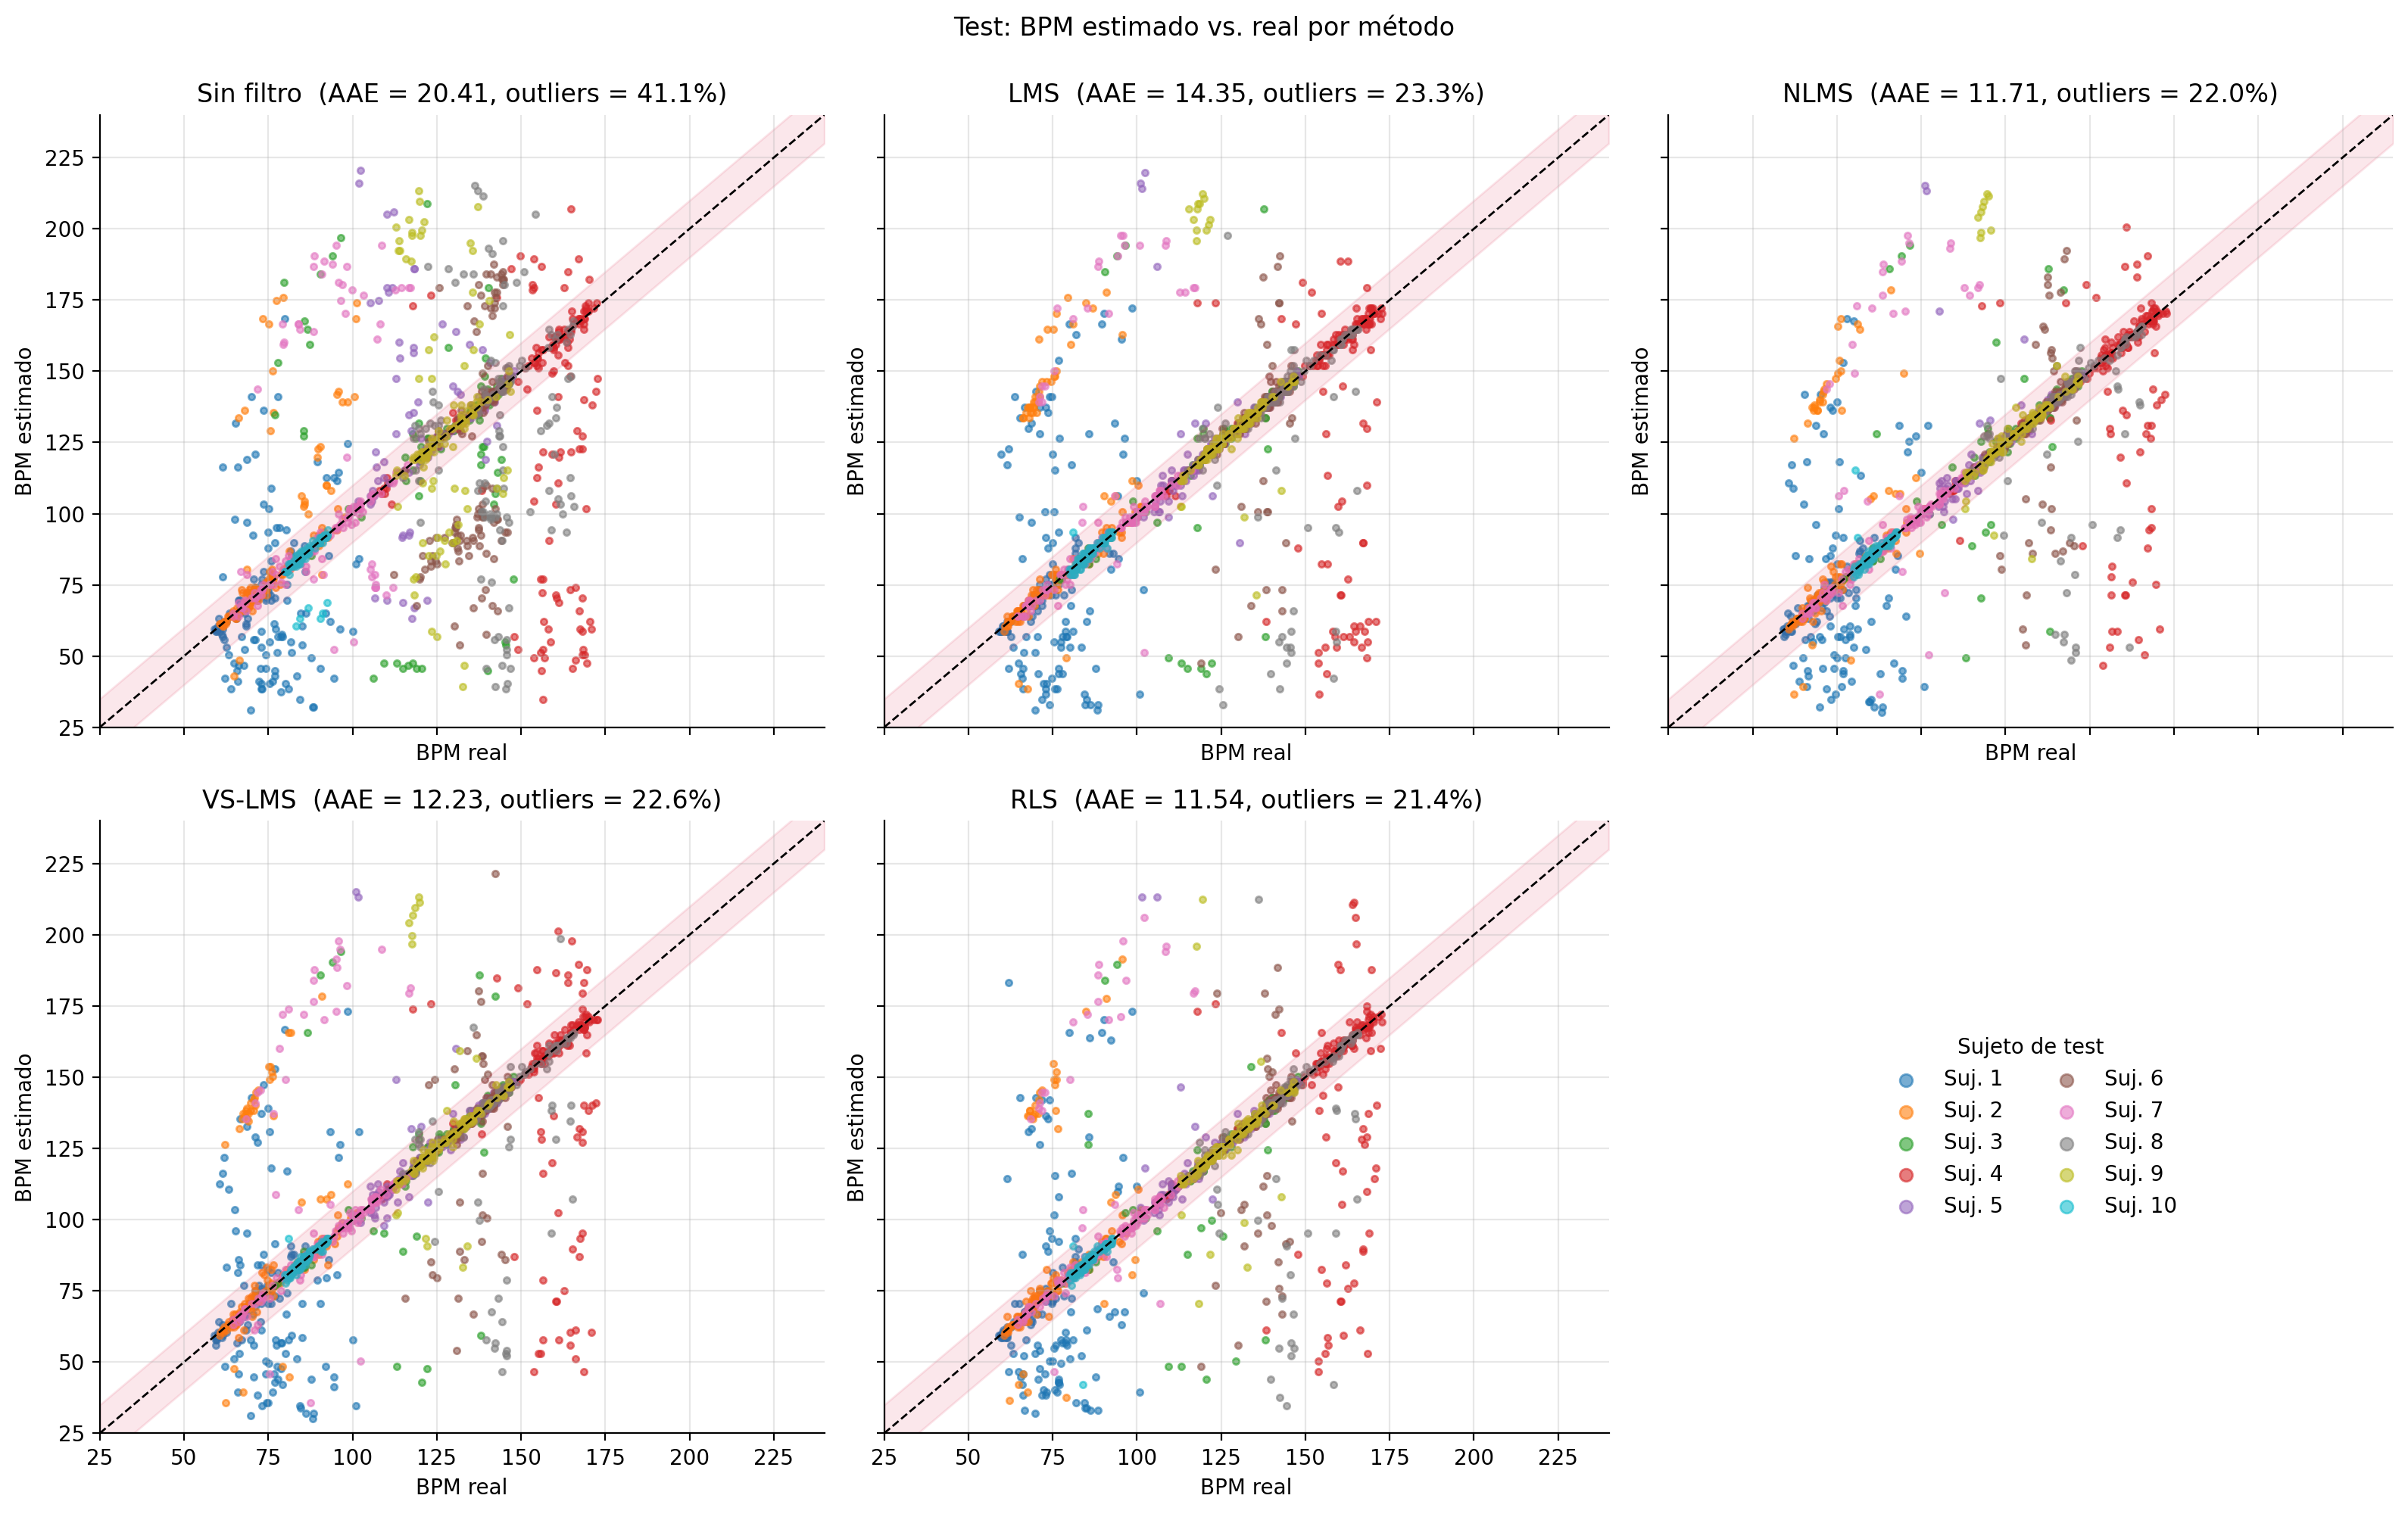
\includegraphics[width=0.64\textwidth]{Figures/02_dispersion_por_metodo.png}
    \caption{BPM estimado frente al real en prueba ($1328$ ventanas) por participante. La banda sombreada indica $\pm 10\text{ BPM}$; todos los filtros comparten grupos de errores en los Sujetos~1, 2, 4 y~8 (esta imagen fue creada utilizando nuestro código).}
    \label{fig:disp}
\end{figure*}

\begin{table}[!t]
    \centering
    \caption{Diferencia media de AAE por \textit{bootstrap} sobre participantes ($\text{método}-\text{RLS}$, $2000$ réplicas).}
    \label{tab:bootstrap}
    \footnotesize
    \begin{tabular}{lccl}
        \toprule
        \textbf{Comparación} & $\Delta$\textbf{AAE} & \textbf{IC 95\%} & \textbf{Conclusión} \\
        \midrule
        Sin filtro $-$ RLS & $+8.81$ & $[3.15,\ 13.59]$ & RLS mejor \\
        LMS $-$ RLS & $+2.80$ & $[1.23,\ 4.57]$ & RLS mejor \\
        NLMS $-$ RLS & $+0.18$ & $[-0.78,\ 1.27]$ & No concluyente \\
        VS-LMS $-$ RLS & $+0.69$ & $[-0.24,\ 1.67]$ & No concluyente \\
        \bottomrule
    \end{tabular}
\end{table}

\begin{figure*}[!t]
    \centering
    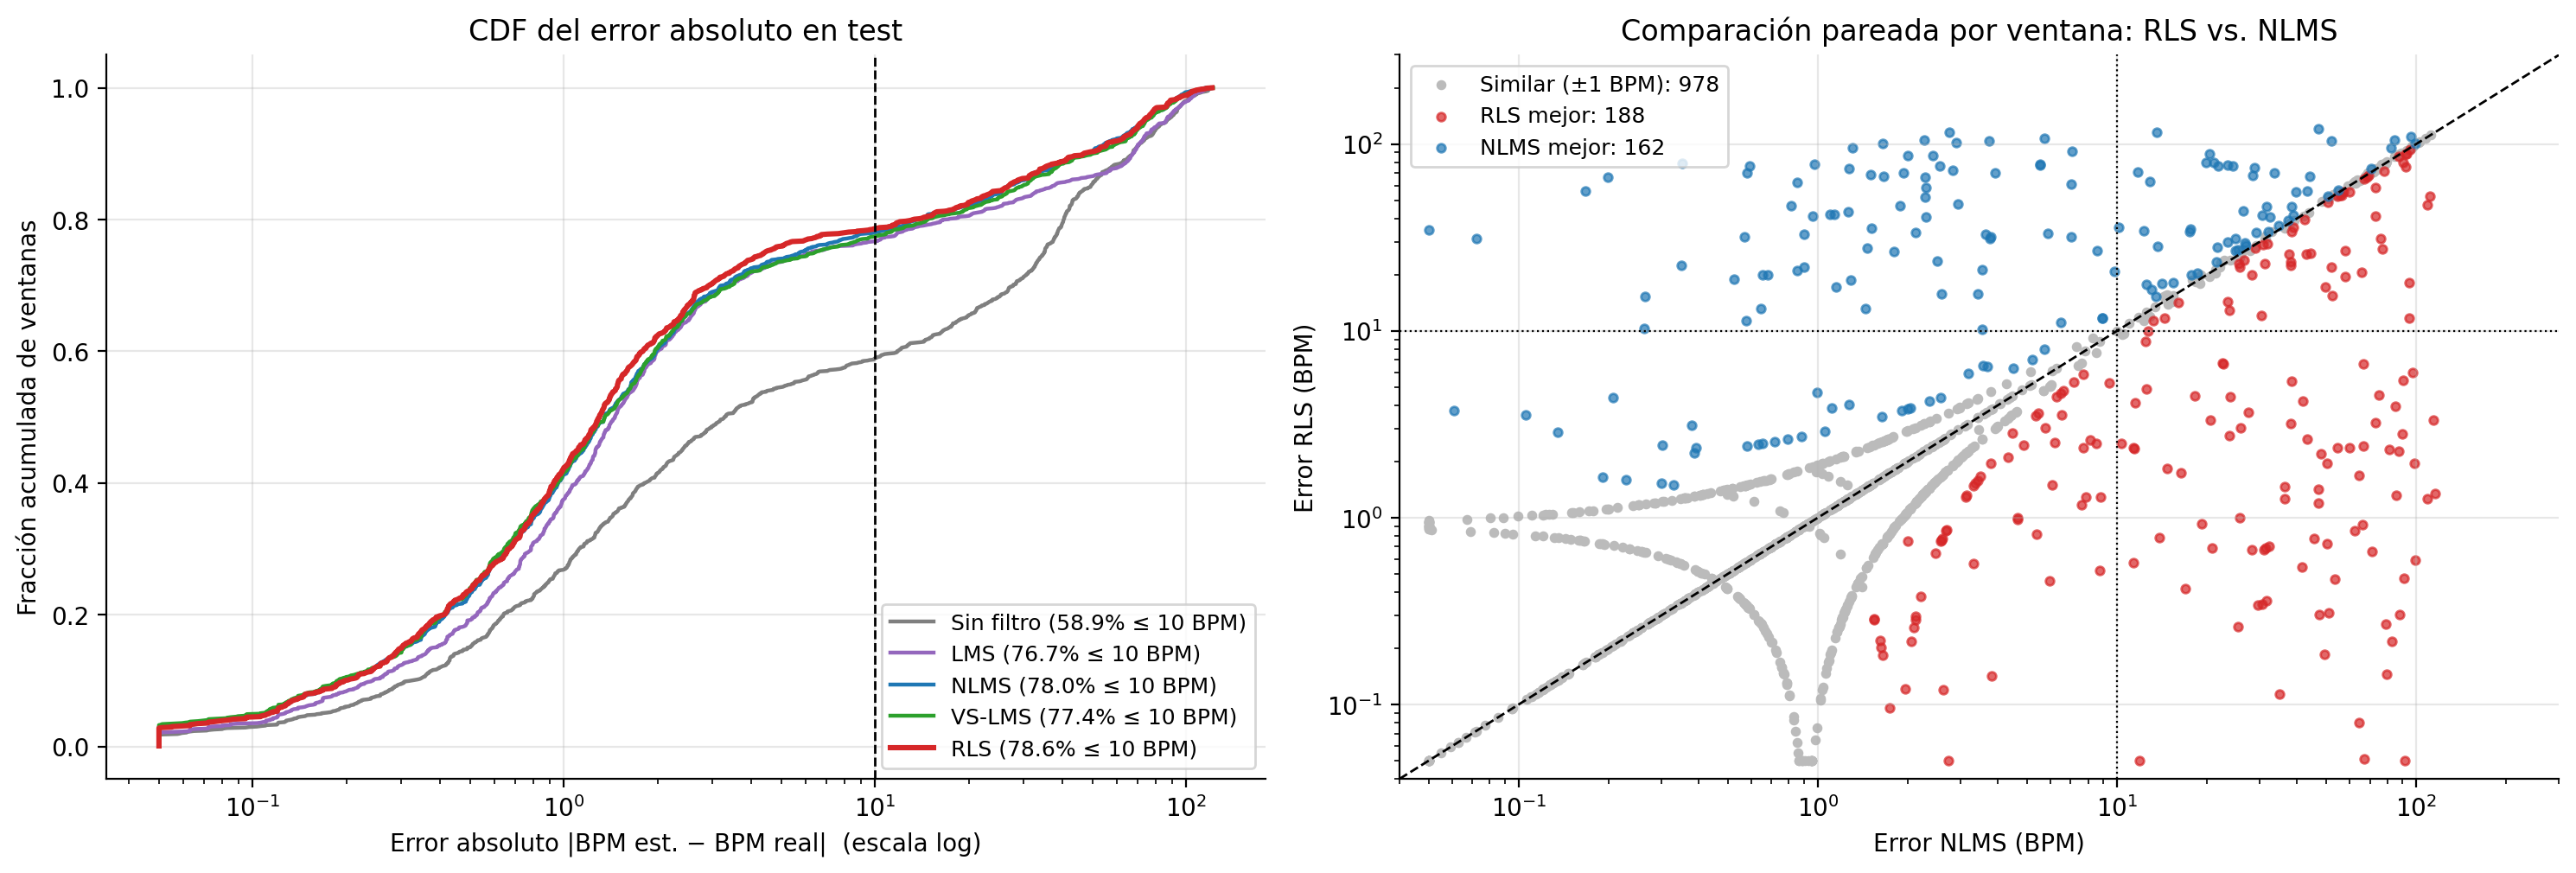
\includegraphics[width=0.65\textwidth]{Figures/03_cdf_y_pareado.png}
    \caption{Izquierda: CDF del error absoluto en prueba (escala logarítmica). Derecha: comparación pareada ventana a ventana entre NLMS reoptimizado y RLS (esta imagen fue creada utilizando nuestro código).}
    \label{fig:cdf}
\end{figure*}

\subsection{Análisis por participante}
\label{sec:res_sujetos}

La Tabla~\ref{tab:test_subjects} detalla el AAE de prueba por participante. RLS supera a NLMS y lidera en $4$ de $10$ sujetos (Sujetos~2, 5, 7 y~9), con reducciones marcadas frente a NLMS en los Sujetos~2 ($16.61\to 14.68$) y~9 ($8.40\to 4.33\text{ BPM}$). NLMS lidera en los Sujetos~1, 3, 4 y~8, LMS en el Sujeto~6 y VS-LMS en el Sujeto~10, concentrándose los mayores errores en los Sujetos~1, 2, 4 y~7 (en los Sujetos~1 y~2 ningún filtro mejora a la base).

\begin{table}[!t]
    \centering
    \caption{AAE (BPM) por participante en el conjunto de prueba (en negrita, el menor error entre filtros).}
    \label{tab:test_subjects}
    \footnotesize
    \setlength{\tabcolsep}{3pt}
    \begin{tabular}{lcccccc}
        \toprule
        \textbf{Sujeto} & \textbf{Vent.} & \textbf{Base} & \textbf{LMS} & \textbf{NLMS} & \textbf{VS-LMS} & \textbf{RLS} \\
        \midrule
        1 & 142 & $19.43$ & $25.68$ & $\mathbf{21.63}$ & $22.34$ & $23.78$ \\
        2 & 137 & $11.15$ & $22.88$ & $16.61$ & $17.70$ & $\mathbf{14.68}$ \\
        3 & 144 & $16.01$ & $7.54$ & $\mathbf{6.58}$ & $7.18$ & $6.62$ \\
        4 & 152 & $31.53$ & $24.32$ & $\mathbf{18.07}$ & $19.76$ & $19.36$ \\
        5 & 101 & $18.55$ & $6.93$ & $5.32$ & $5.27$ & $\mathbf{4.49}$ \\
        6 & 157 & $24.83$ & $\mathbf{7.43}$ & $8.28$ & $7.89$ & $8.35$ \\
        7 & 132 & $21.55$ & $16.23$ & $15.29$ & $16.94$ & $\mathbf{14.84}$ \\
        8 & 142 & $28.47$ & $14.60$ & $\mathbf{10.68}$ & $10.93$ & $11.76$ \\
        9 & 121 & $23.49$ & $10.79$ & $8.40$ & $7.86$ & $\mathbf{4.33}$ \\
        10 & 100 & $2.13$ & $1.05$ & $1.23$ & $\mathbf{0.89}$ & $1.27$ \\
        \bottomrule
    \end{tabular}
\end{table}

\subsection{Casos de estudio}
\label{sec:res_casos}

La Fig.~\ref{fig:casos} analiza tres ventanas del Sujeto~4: la \#481 (\textit{outlier} de~\cite{informe1}), la \#484 (mayor ganancia de RLS sobre NLMS) y la \#477 (mayor pérdida). En la \#481 (real $168.6\text{ BPM}$) ningún filtro acierta (sin filtro $140.1$, NLMS $142.8$, RLS $138.2\text{ BPM}$). En la \#484 (real $166.1$) NLMS deja dominante un pico de movimiento en $50.4\text{ BPM}$, mientras RLS lo suprime y estima $164.8\text{ BPM}$. En la \#477 (real $168.4$) ocurre lo inverso: NLMS acierta ($170.3$) y RLS deja dominar un pico en $53.1\text{ BPM}$ frente al latido atenuado. En estas ventanas compiten picos en $40$--$80\text{ BPM}$ contra el pico cardíaco, de modo que la selección de máximo único provoca saltos de $>100\text{ BPM}$.

\begin{figure*}[!t]
    \centering
    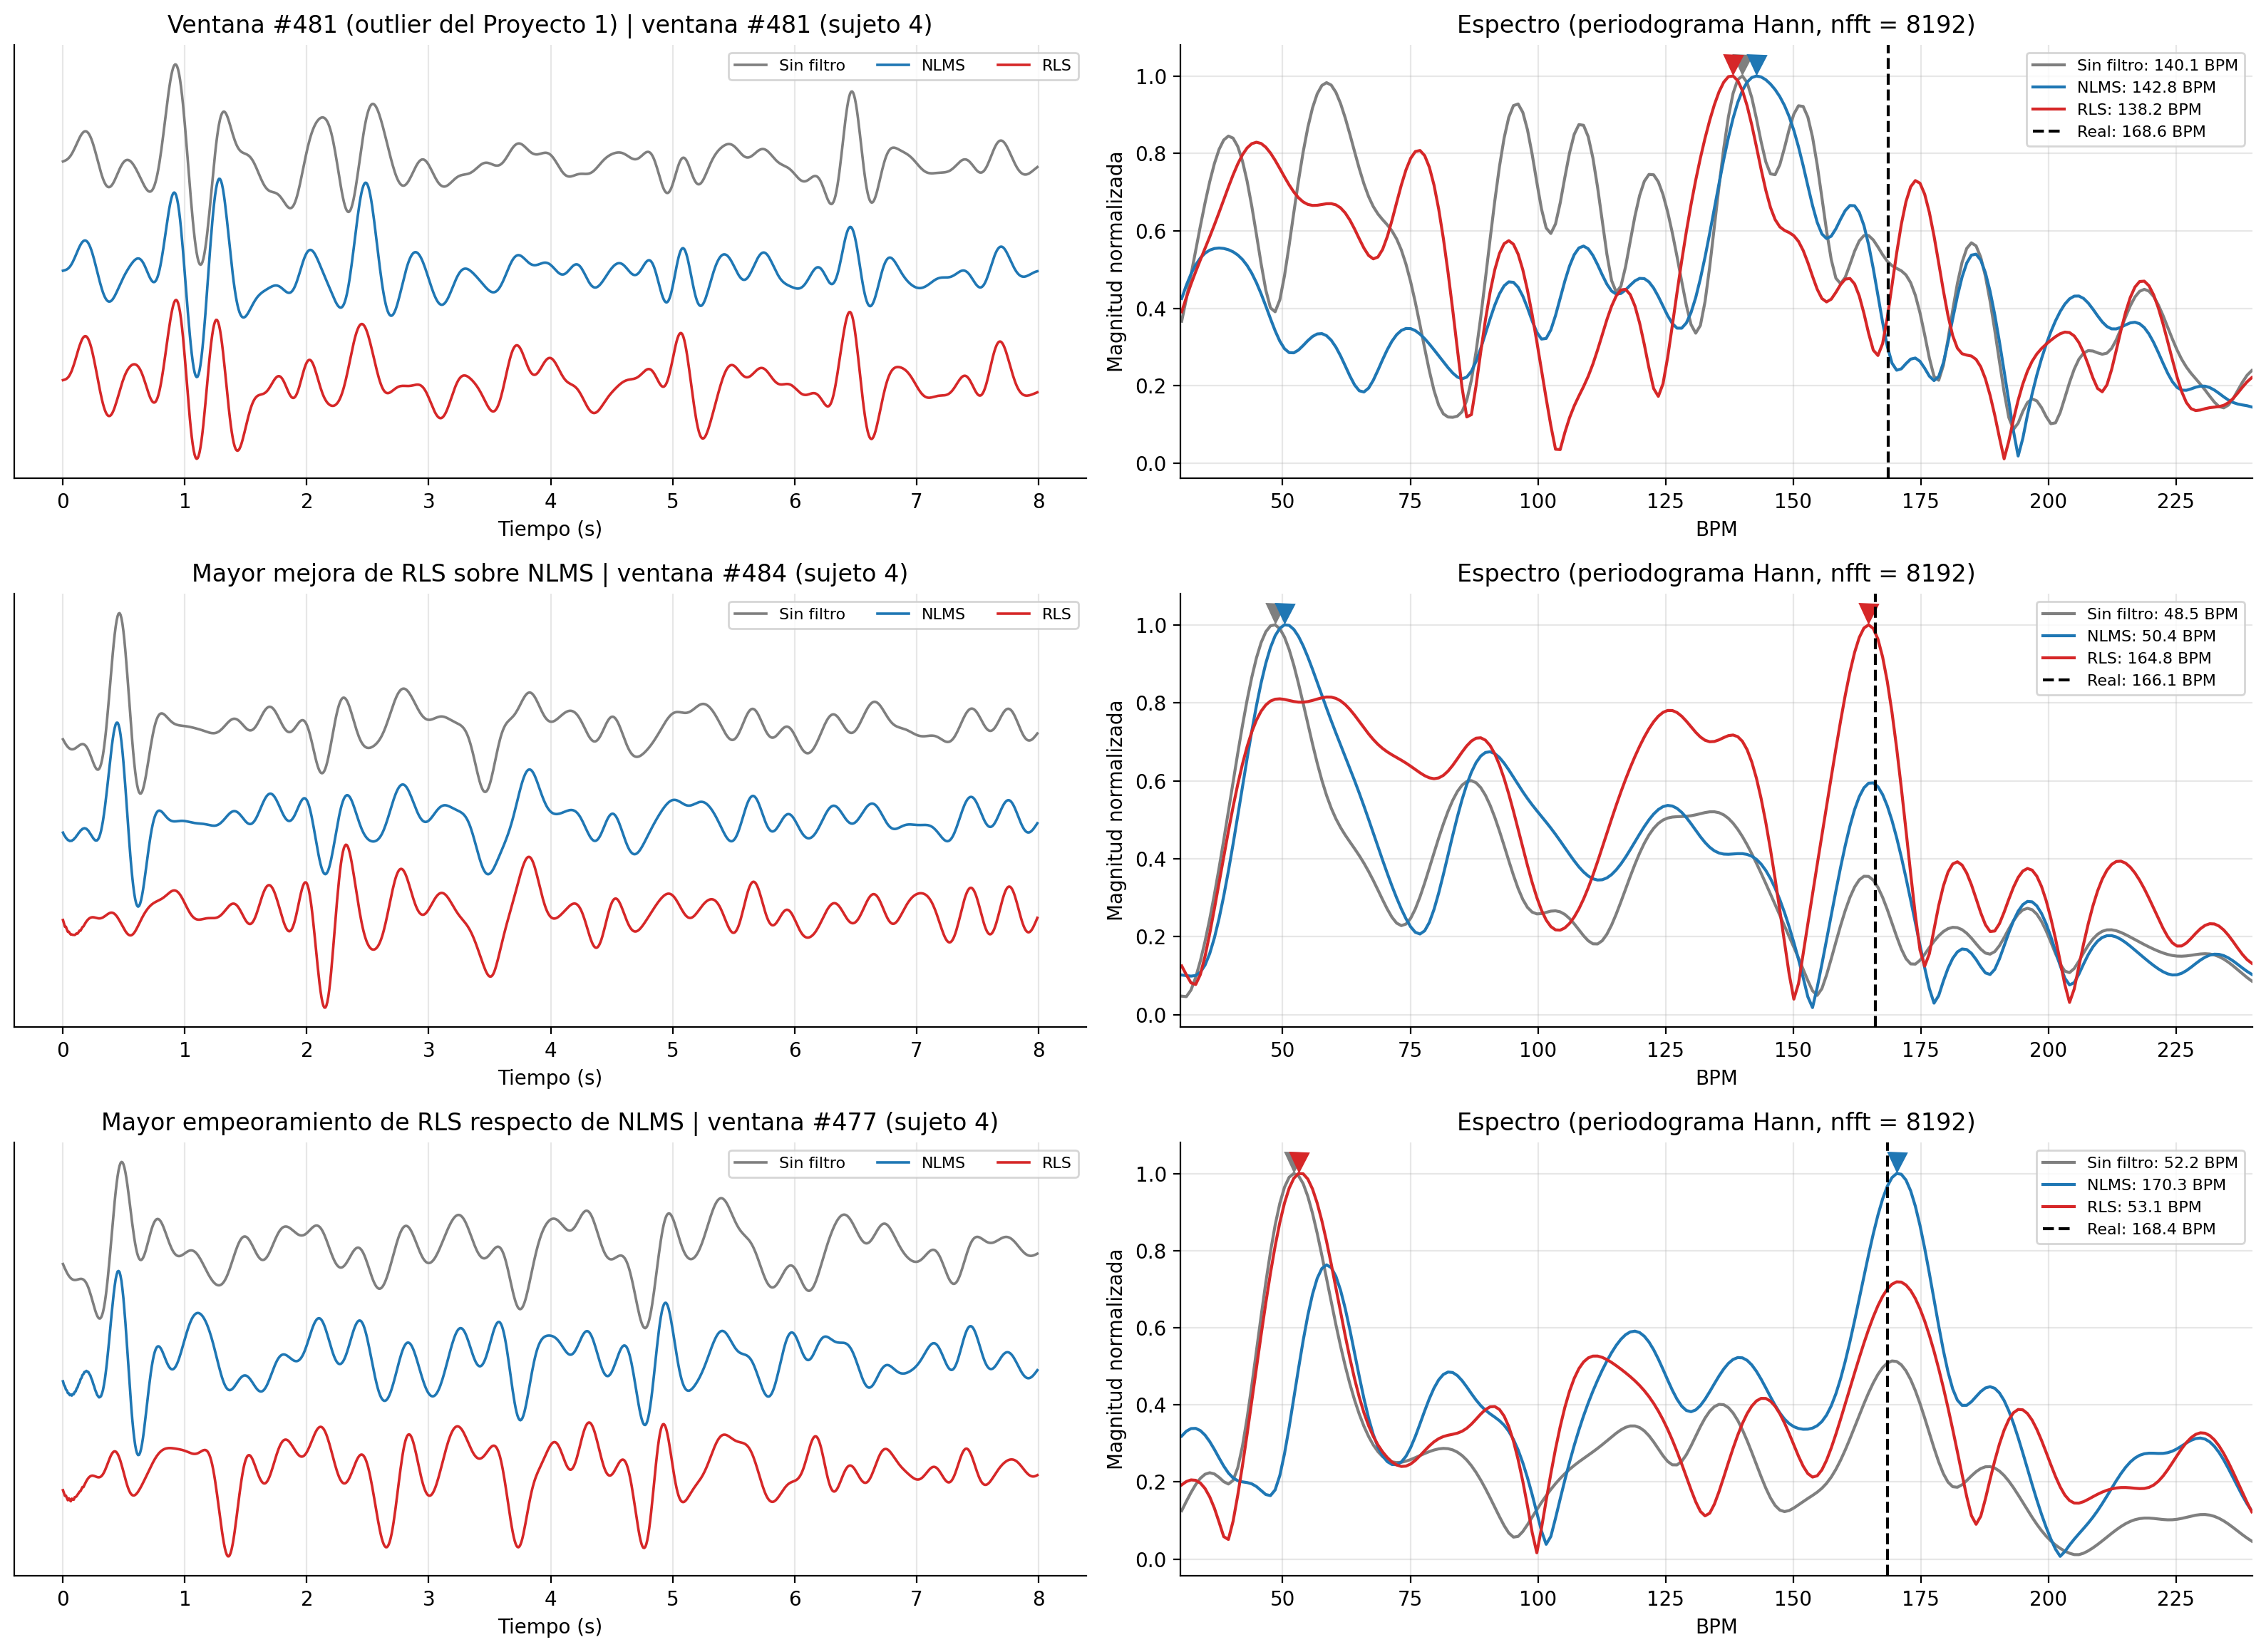
\includegraphics[width=0.63\textwidth]{Figures/06_casos_concretos.png}
    \caption{Casos de estudio en el Sujeto~4: \#481 (\textit{outlier} de~\cite{informe1}), \#484 (mayor mejora de RLS) y \#477 (mayor empeoramiento frente a NLMS). Izquierda: señales normalizadas; derecha: espectros Hann ($\text{NFFT}=8192$) con BPM real en línea punteada (esta imagen fue creada utilizando nuestro código).}
    \label{fig:casos}
\end{figure*}

\subsection{Análisis de filtros adaptativos: modos, aprendizaje, estabilidad y costo}
\label{sec:res_conv}

La Fig.~\ref{fig:modos} caracteriza la dinámica interna de los filtros sobre $150$ ventanas de prueba. En el panel~(a), el espectro de autovalores de $\hat{\mathbf{R}}$ bajo sobremuestreo denso ($D=1, M=15$) colapsa por debajo de $10^{-9}$ ($\chi\approx 2.2\times 10^{16}$), generando en LMS constantes de tiempo modales $\tau_i=1/(2\mu\lambda_i f_s)$ sumamente dispares: mientras el modo dominante converge en $\tau_1=0.33\text{ s}$, el quinto modo requiere $\tau_5=10.01\text{ s}$ y el décimo supera $10^4\text{ s}$, dejando modos secundarios sin converger dentro de la ventana de $8\text{ s}$. La dilatación ($D=3, M=8$) comprime seis órdenes de magnitud el espectro ($\chi\approx 4.0\times 10^{10}$), y sumar la previa $\delta_0=239.3$ ($2.52\%$ de $\lambda_{\max,\text{med}}=9488$) reduce el condicionamiento efectivo a $\chi_{\text{ef}}\approx 41$ sin sesgar los modos dominantes.

El panel~(b) muestra las curvas de aprendizaje $J(n)=\operatorname{mediana}[e^2[n]]$ con arranque en frío ($\text{WS}=0$). RLS alcanza su régimen estacionario ($-5.68\text{ dB}$) exactamente en el umbral teórico $2L/f_s=0.38\text{ s}$ ($-5.79\text{ dB}$ en $1\text{ s}$, $\mathcal{M}_{\text{RLS}}=0.64\%$), mientras NLMS ($-3.17\text{ dB}$ a $0.38\text{ s}$, $-4.88\text{ dB}$ en $1\text{ s}$) y LMS ($-4.51\text{ dB}$ a $0.38\text{ s}$) exhiben mayor transitorio y retardo hacia el estado estacionario; por su parte, el RLS ingenuo ($D=1,\lambda=0.98,\delta=0.01$) cae a $-33.41\text{ dB}$ a $0.38\text{ s}$ por sobreajuste extremo del pulso cardíaco. En el panel~(c), esa amplificación por $1/\lambda_i$ y $\lambda^{-n}$ en el subespacio nulo hace divergir exponencialmente la norma $\lVert\mathbf{w}[n]\rVert_2$ del RLS ingenuo hasta una mediana de $3.54\times 10^4$ ($P_{95}=8.03\times 10^4$) al final de la ventana, mientras RLS regularizado ($0.382$, $P_{95}=0.538$), LMS ($0.277$) y NLMS ($0.158$) permanecen estrictamente acotados.

Con precalentamiento activo (Fig.~\ref{fig:conv}), RLS ($\text{WS}=0.25$) parte atenuado en $\approx -8.5\text{ dB}$ a $0.3\text{ s}$ y todos los filtros estabilizan entre $-5$ y $-6\text{ dB}$ tras el latido residual, validando la expectativa~(i). En costo mediano sobre las $1328$ ventanas de prueba (dos canales y fusión), RLS tarda $18.6\text{ ms}$ frente a $14.2\text{ ms}$ de NLMS ($1.3\times$), $15.2\text{ ms}$ de VS-LMS y $11.2\text{ ms}$ de LMS ($24.86\text{ s}$ frente a $19.28\text{ s}$ de NLMS en el total). Compartir $\mathbf{P}(n)$ y operar con $L=24$ pesos (frente a $L=102$ en NLMS) mantiene la latencia por debajo del $1\%$ del avance entre ventanas ($2000\text{ ms}$), viable en tiempo real.

\begin{figure*}[!t]
    \centering
    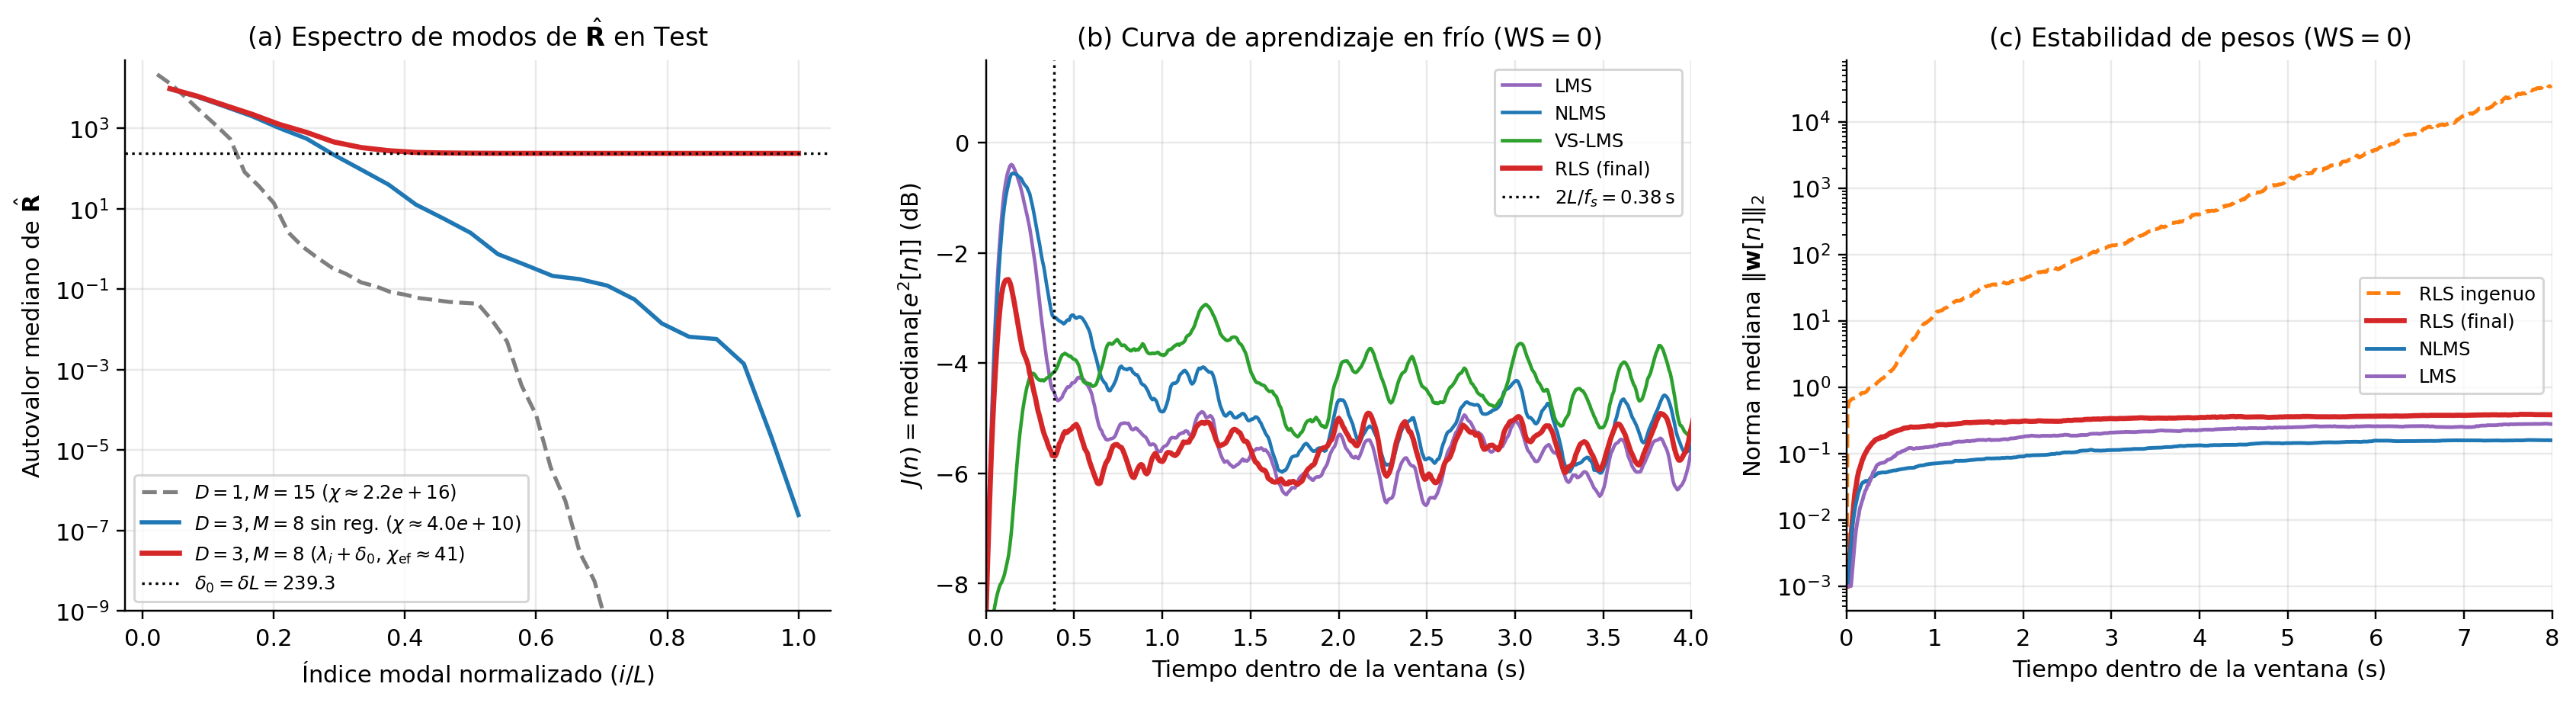
\includegraphics[width=0.61\textwidth]{Figures/09_modos_y_aprendizaje_test.png}
    \caption{Diagnóstico adaptativo en $150$ ventanas de prueba ($\text{WS}=0$): (a) espectro modal de $\hat{\mathbf{R}}$; (b) curva de aprendizaje en frío con marcador teórico $2L/f_s=0.38\text{ s}$; (c) estabilidad de $\lVert\mathbf{w}[n]\rVert_2$ mostrando la deriva del RLS ingenuo (esta imagen fue creada utilizando nuestro código).}
    \label{fig:modos}
\end{figure*}

\begin{figure*}[!t]
    \centering
    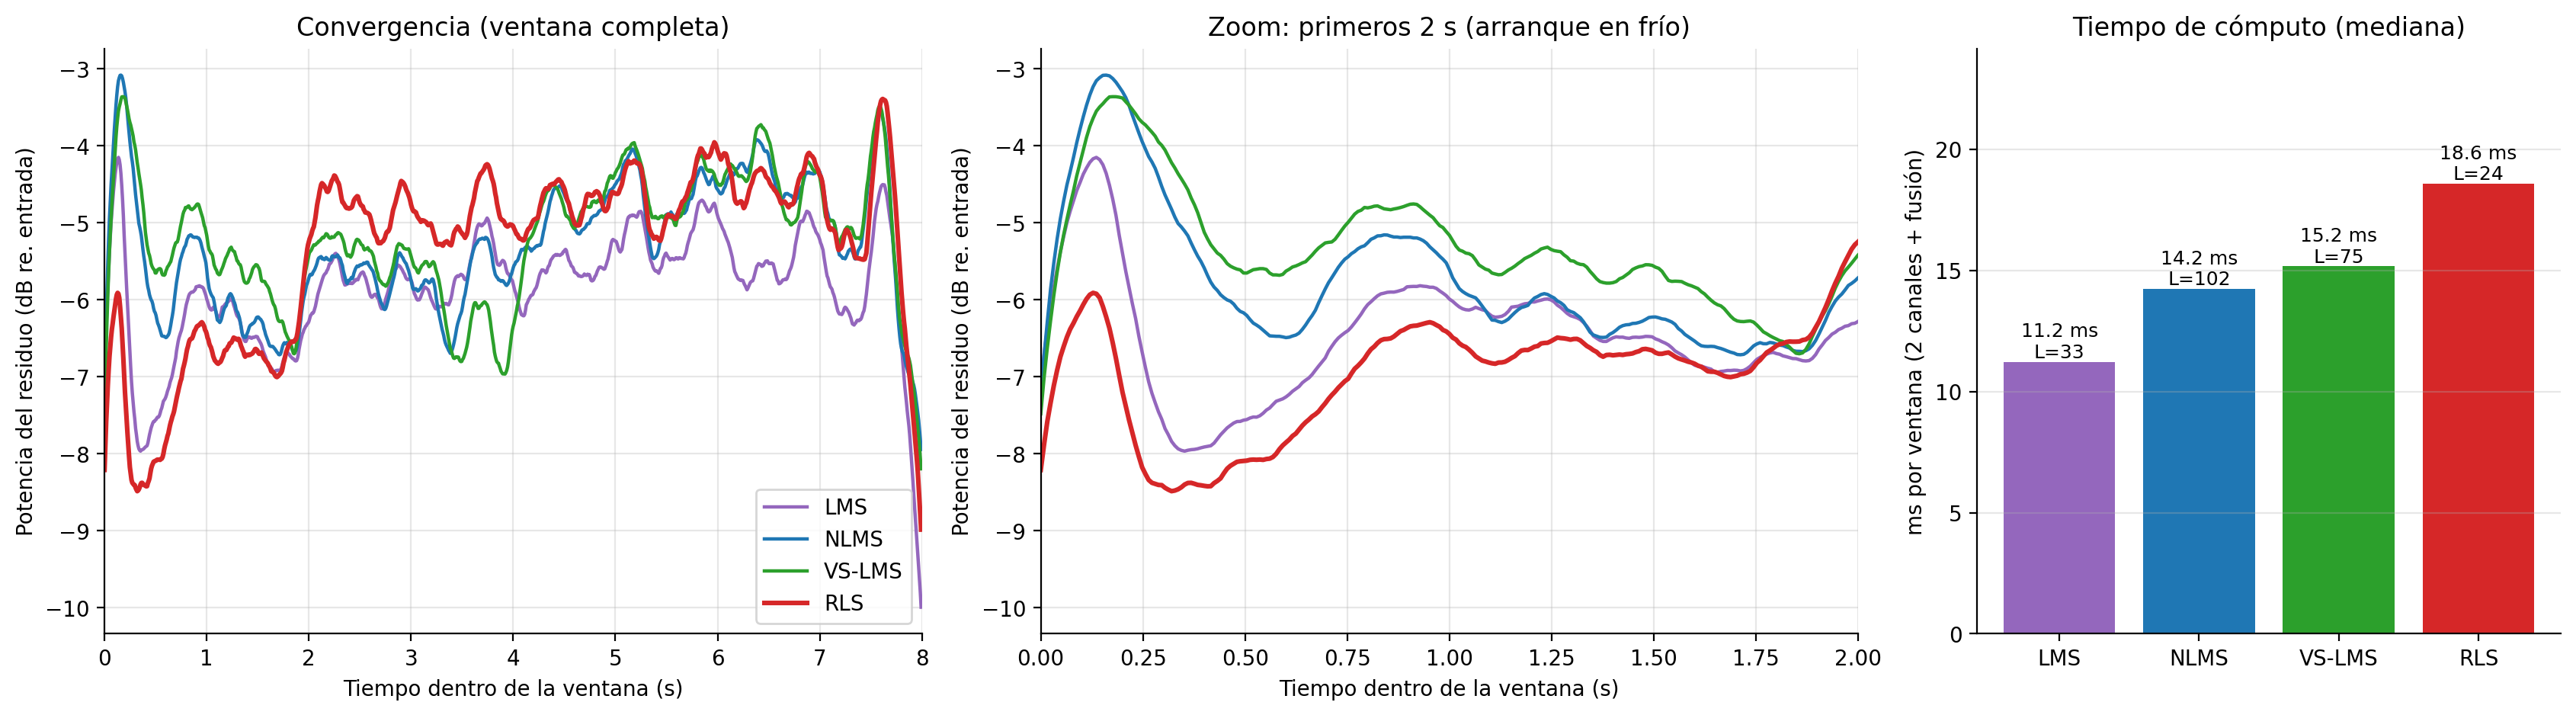
\includegraphics[width=0.59\textwidth]{Figures/05_convergencia_y_costo.png}
    \caption{Operación final con \textit{warm start}: potencia residual mediana en $150$ ventanas de prueba (izquierda y centro) y costo computacional mediano en prueba junto al total de pesos $L$ (derecha) (esta imagen fue creada utilizando nuestro código).}
    \label{fig:conv}
\end{figure*}

\subsection{Ablación diagnóstica y sensibilidad de RLS en prueba}
\label{sec:ablacion}

Para cuantificar la contribución de cada componente estructural evaluamos $16$ variantes sobre un subconjunto estratificado de $200$ ventanas de prueba ($20$ aleatorias por participante, periodograma común Hann $8192$; base sin filtro $\text{AAE}=19.72\text{ BPM}$, $\text{MedAE}=2.76\text{ BPM}$, \textit{outliers} $=40.0\%$), resumidas en la Tabla~\ref{tab:ablacion} y la Fig.~\ref{fig:sens}:

\begin{table}[!t]
    \centering
    \caption{Ablación diagnóstica sobre $200$ ventanas estratificadas de prueba (Hann $8192$; base $19.72\text{ BPM}$). «Estruc.\ RLS» indica $D=3$, Huber $c=2.660$ y $\text{WS}=0.25$.}
    \label{tab:ablacion}
    \footnotesize
    \setlength{\tabcolsep}{2pt}
    \begin{tabular}{lccc}
        \toprule
        \textbf{Variante} & \textbf{AAE} & \textbf{MedAE} & \textbf{Outliers} \\
        \midrule
        LMS Proy.\ 1 ($D=1, M=11$) & $13.81$ & $1.55$ & $22.0\%$ \\
        LMS + estruc.\ RLS ($D=3, M=11$) & $13.21$ & $1.57$ & $22.5\%$ \\
        NLMS Proy.\ 1 ($D=1, M=22$) & $12.74$ & $1.41$ & $23.5\%$ \\
        NLMS + estruc.\ RLS ($D=3, M=8$) & $12.44$ & $1.55$ & $23.5\%$ \\
        NLMS reoptimizado ($D=2, M=34$) & $11.51$ & $1.62$ & $22.5\%$ \\
        VS-LMS Proy.\ 1 ($D=1, M=18$) & $16.18$ & $1.73$ & $28.0\%$ \\
        VS-LMS + estruc.\ RLS ($D=3, M=8$) & $16.01$ & $1.76$ & $26.5\%$ \\
        VS-LMS reoptimizado ($D=2, M=25$) & $11.44$ & $1.57$ & $22.0\%$ \\
        \midrule
        RLS ingenuo ($D=1,\lambda=.98,\delta=.01$) & $23.83$ & $3.98$ & $42.0\%$ \\
        \textbf{RLS final} ($D=3, M=8$) & $\mathbf{10.96}$ & $1.49$ & $22.0\%$ \\
        RLS final sin dilatación ($D=1, M=22$) & $10.86$ & $1.49$ & $\mathbf{21.5\%}$ \\
        RLS final sin Huber & $10.96$ & $1.50$ & $22.0\%$ \\
        RLS final sin carga diagonal & $11.19$ & $1.49$ & $22.0\%$ \\
        RLS final sin olvido ($\lambda=1$) & $11.63$ & $1.50$ & $22.5\%$ \\
        RLS final + \textit{warm start} ($35\%$) & $11.26$ & $1.49$ & $22.5\%$ \\
        RLS final con $\delta=0.05$ & $20.42$ & $2.61$ & $35.5\%$ \\
        \bottomrule
    \end{tabular}
\end{table}

\begin{figure*}[!t]
    \centering
    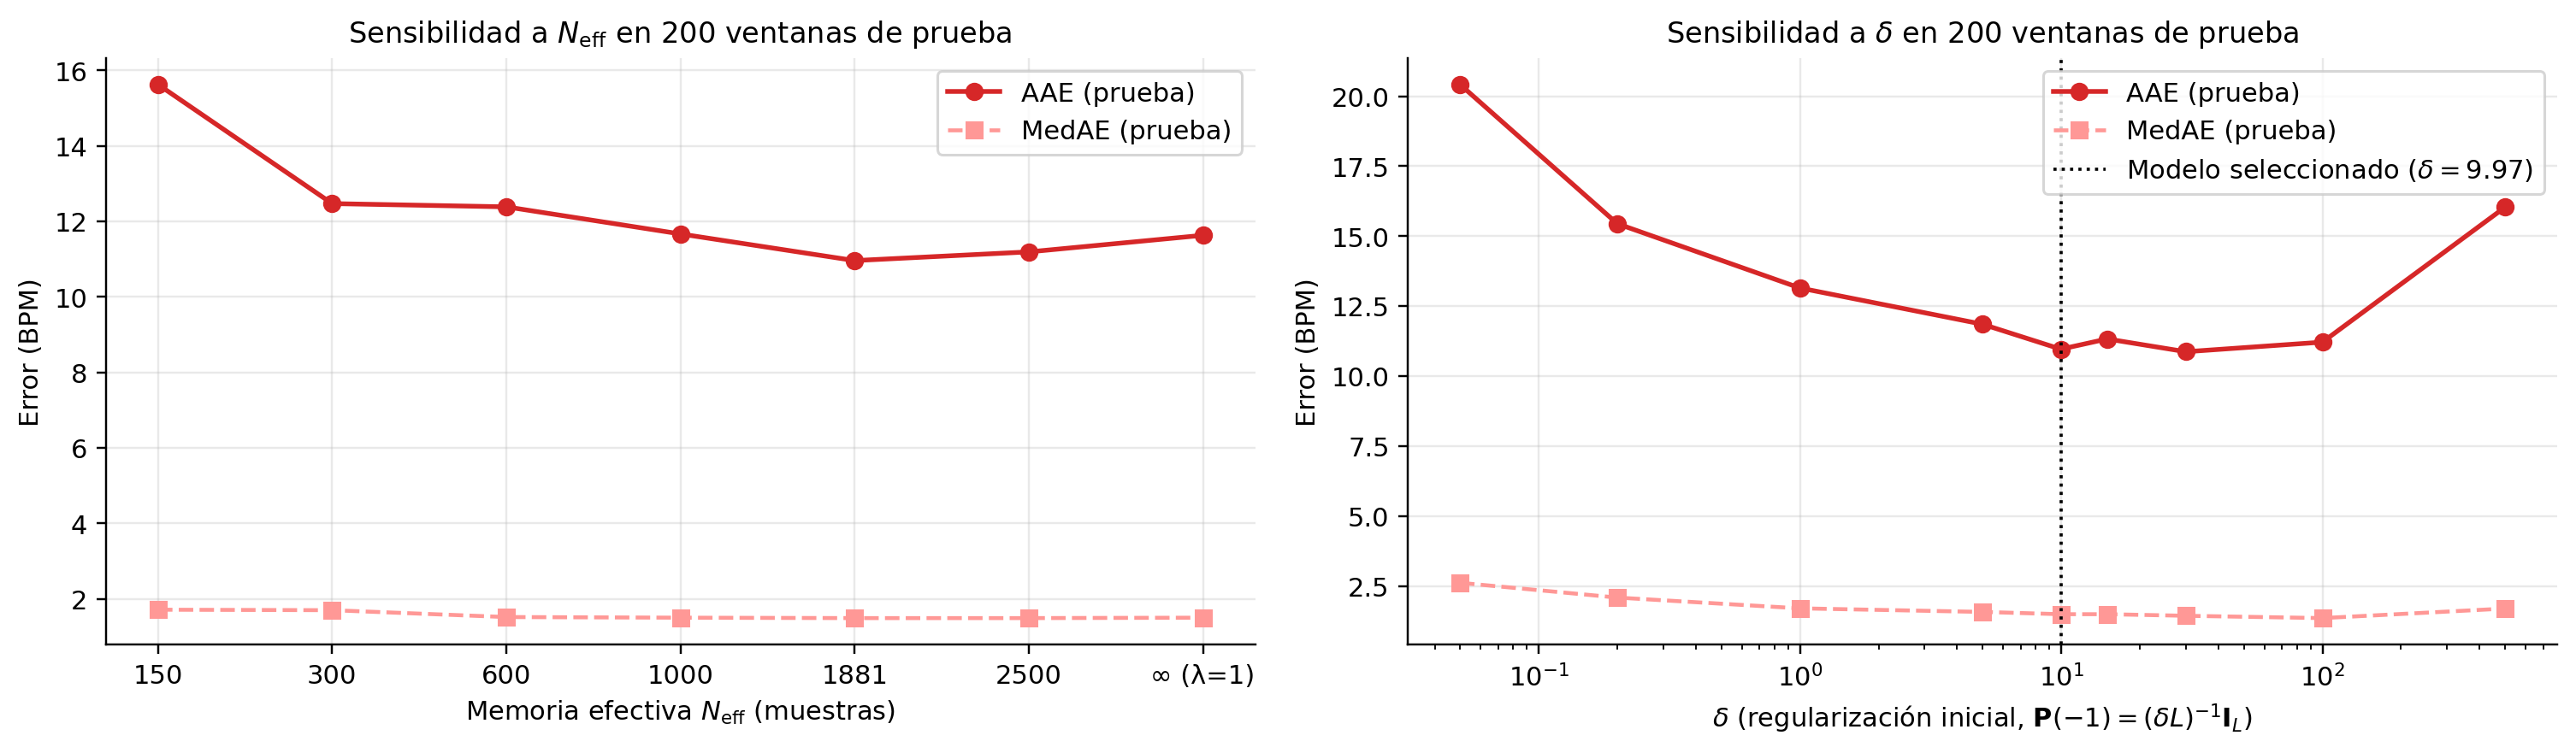
\includegraphics[width=0.55\textwidth]{Figures/08_sensibilidad_RLS_test.png}
    \caption{Sensibilidad de RLS en $200$ ventanas estratificadas de prueba respecto de $N_{\text{eff}}$ (izquierda) y de $\delta$ con $\mathbf{P}(-1)=(\delta L)^{-1}\mathbf{I}_L$ (derecha) (esta imagen fue creada utilizando nuestro código).}
    \label{fig:sens}
\end{figure*}

\begin{enumerate}
    \item \textbf{El RLS ingenuo degrada respecto de no filtrar:} con parámetros de libro ($\delta=0.01,\lambda=0.98,D=1$) alcanza $23.83\text{ BPM}$ ($42.0\%$ \textit{outliers}), peor que no filtrar ($19.72\text{ BPM}$) y detrás de todas las variantes LMS ($11.44$--$16.18\text{ BPM}$). El RLS final reduce el AAE a $10.96\text{ BPM}$ ($22.0\%$ \textit{outliers}).
    \item \textbf{Motivación física de $\delta=9.97$:} a primera vista, $\delta=9.972$ ($\delta_0=\delta L\approx 239.3$ en $\mathbf{P}(-1)=\delta_0^{-1}\mathbf{I}_L$) parece excesivo frente a la regla clásica $\delta_0\approx 0.01\sigma_a^2$. Sin embargo, en~(\ref{eq:costo_rls}) la matriz $\hat{\mathbf{R}}(n)$ es una suma \emph{sin dividir por $N$}: sobre $1000$ muestras normalizadas en prueba, para $(D=3,M=8,L=24)$ su traza mediana es $23{,}930$ y su autovalor máximo mediano es $\lambda_{\max}(\hat{\mathbf{R}})=9{,}488$ ($\chi\approx 4.0\times 10^{10}$). Así, $\delta_0=239.3$ equivale al $2.52\%$ de $\lambda_{\max}$: apenas sesga las direcciones dominantes del movimiento, pero amortigua los autovalores colineales del subespacio nulo vía~(\ref{eq:desvio_l1}), en concordancia con Moustakides~\cite{moustakides1997rls} para baja SNR. Bajar $\delta$ a $0.05$ dispara el error a $20.42\text{ BPM}$; en la Fig.~\ref{fig:sens} (derecha) la curva en U desciende hasta un mínimo en $\delta=30$ ($10.87\text{ BPM}$, con $10.96$ en $\delta=9.972$) y repunta por sobre-sesgo ($\mathbf{w}\to\mathbf{0}$) en $\delta=100$ ($11.21$) y $\delta=500$ ($16.04\text{ BPM}$).
    \item \textbf{Dilatación como opción de acondicionamiento y cómputo:} a apertura fija ($\approx 168\text{ ms}$) en prueba, $D=1$ ($M=22,L=66$) y $D=2$ ($M=11,L=33$) logran $10.86$ y $10.84\text{ BPM}$ ($\chi\approx 2.8\times 10^{16}$ y $1.0\times 10^{16}$), mientras $D=3$ ($M=8,L=24$) obtiene $10.96\text{ BPM}$ ($\chi\approx 4.3\times 10^{10}$) y $D=4$ ($M=6,L=18$) $11.20\text{ BPM}$ ($\chi\approx 1.6\times 10^{7}$). Así, activas $\delta_0=\delta L$ y la carga diagonal (cuya supresión eleva el error de $10.96$ a $11.19\text{ BPM}$), $D>1$ no es indispensable en precisión puntual, pero comprime $\mathbf{P}(n)$ en $7.6\times$ menos entradas ($L=66\to 24$) manteniendo la convergencia en $2L=48$ muestras y favoreciendo la generalización en CV. Quitar Huber en este subconjunto deja el AAE casi inalterado ($10.96\text{ BPM}$, $\text{MedAE } 1.49\to 1.50$) y $\text{WS}=0.35$ da $11.26\text{ BPM}$.
    \item \textbf{Memoria larga frente a olvido rápido:} la Fig.~\ref{fig:sens} (izquierda) muestra que $N_{\text{eff}}<600$ degrada con fuerza el error en prueba ($15.63\text{ BPM}$ en $N_{\text{eff}}=150$, $12.47$ en $300$, $12.39$ en $600$), mientras un olvido suave en torno al valor seleccionado ($N_{\text{eff}}=1881.4$, $10.96\text{ BPM}$) supera levemente al RLS sin olvido ($\lambda=1$, $11.63\text{ BPM}$), mostrando una utilidad moderada de la expectativa~(ii) en $8\text{ s}$ sin sacrificar estabilidad.
\end{enumerate}

\begin{figure*}[!t]
    \centering
    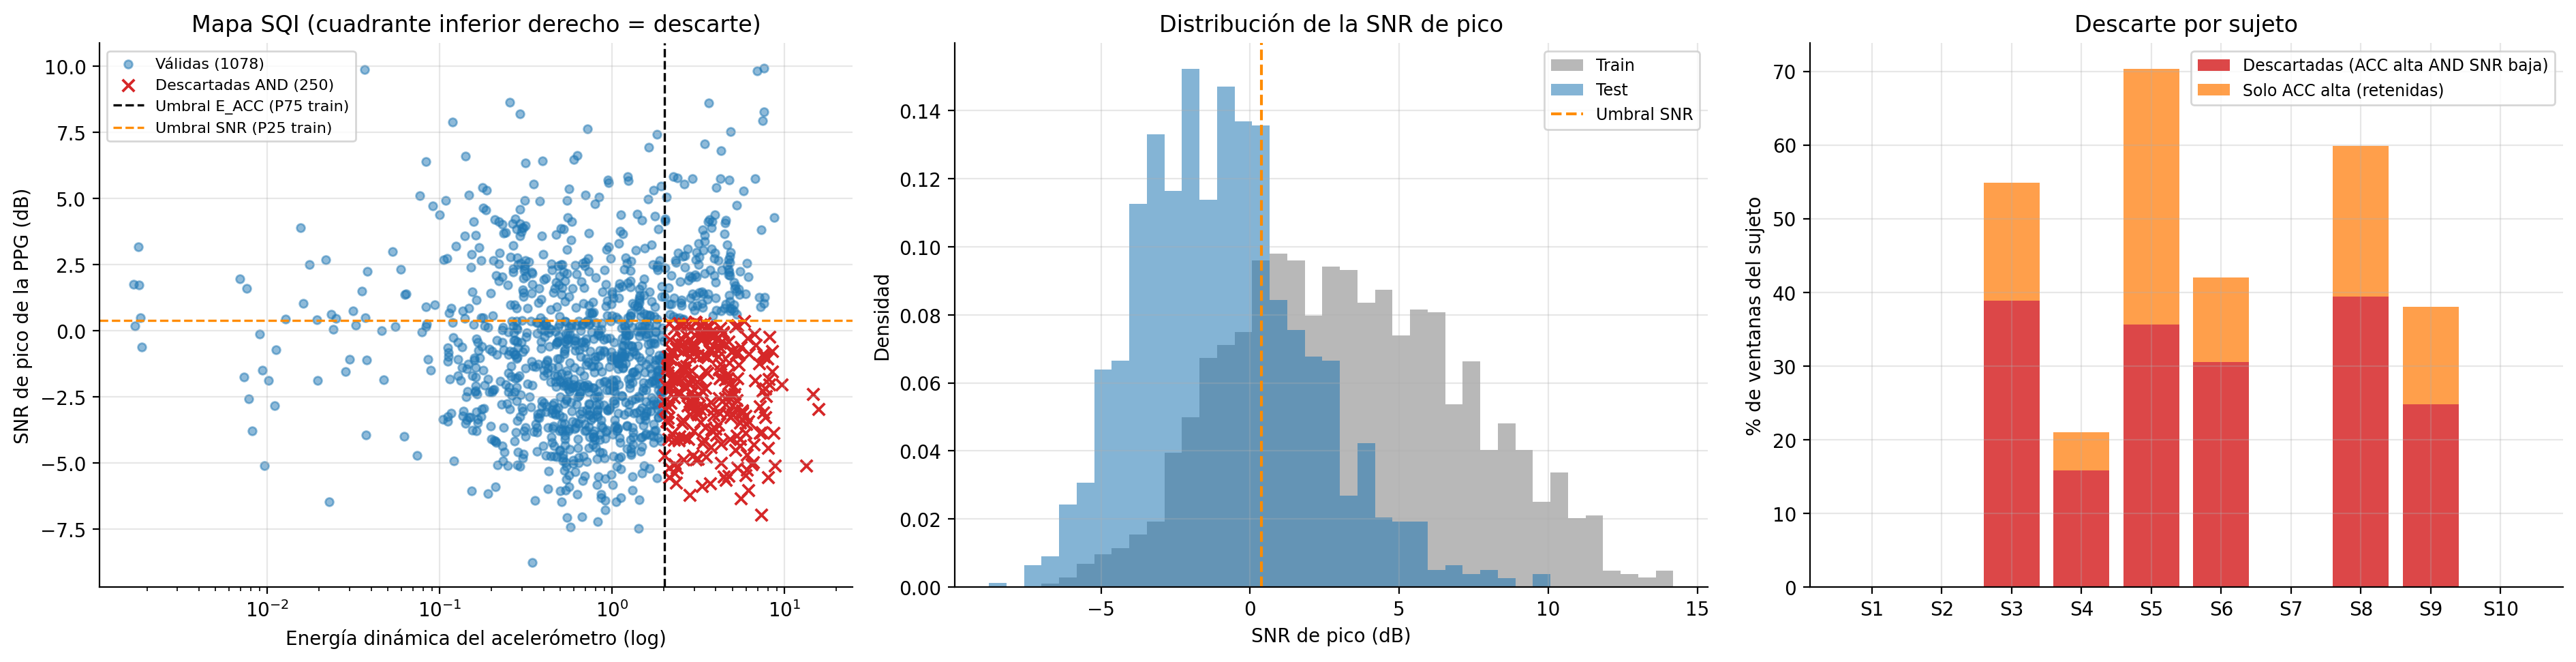
\includegraphics[width=0.59\textwidth]{Figures/01_diagnostico_sqi.png}
    \caption{Diagnóstico del SQI dual en prueba: mapa $(E_{\text{ACC}}, \text{SNR}_{\text{pico}})$ con $250$ descartes (izquierda), desplazamiento de $\text{SNR}_{\text{pico}}$ frente a entrenamiento (centro) y porcentaje descartado por sujeto (derecha) (esta imagen fue creada utilizando nuestro código).}
    \label{fig:sqi_diag}
\end{figure*}

\subsection{Control de calidad (SQI) y regímenes de movimiento}
\label{sec:res_sqi}

En prueba, la compuerta AND ($E_{\text{ACC}}>2.006$ y $\text{SNR}_{\text{pico}}<0.39\text{ dB}$) descartó $250/1328$ ventanas ($18.83\%$) y retuvo $1078$ ($81.17\%$). La Fig.~\ref{fig:sqi_diag} evidencia el corrimiento de $\text{SNR}_{\text{pico}}$ entre entrenamiento y prueba (mediana $3.10$ frente a $-1.05\text{ dB}$), justificando los percentiles, y muestra que los descartes se concentran en los Sujetos~3, 4, 5, 6, 8 y~9 ($0\%$ en los Sujetos~1, 2, 7 y~10). Cuantitativamente (Tabla~\ref{tab:sqi}), el SQI solo mejora a la base sin filtrar ($20.41\to 19.11\text{ BPM}$), mientras \emph{empeora} el AAE de las retenidas en todos los filtros (RLS sube a $12.03$ y NLMS a $12.11\text{ BPM}$), sin superar al azar ($p\in[0.868,0.949]$). En la grilla $P_{65}$--$P_{85}\times P_{15}$--$P_{35}$ ($12.6\%$--$25.5\%$ de descarte), ambos filtros quedan prácticamente empatados ($\text{NLMS}-\text{RLS}$ entre $-0.31$ y $+0.14\text{ BPM}$).

\begin{figure*}[!t]
    \centering
    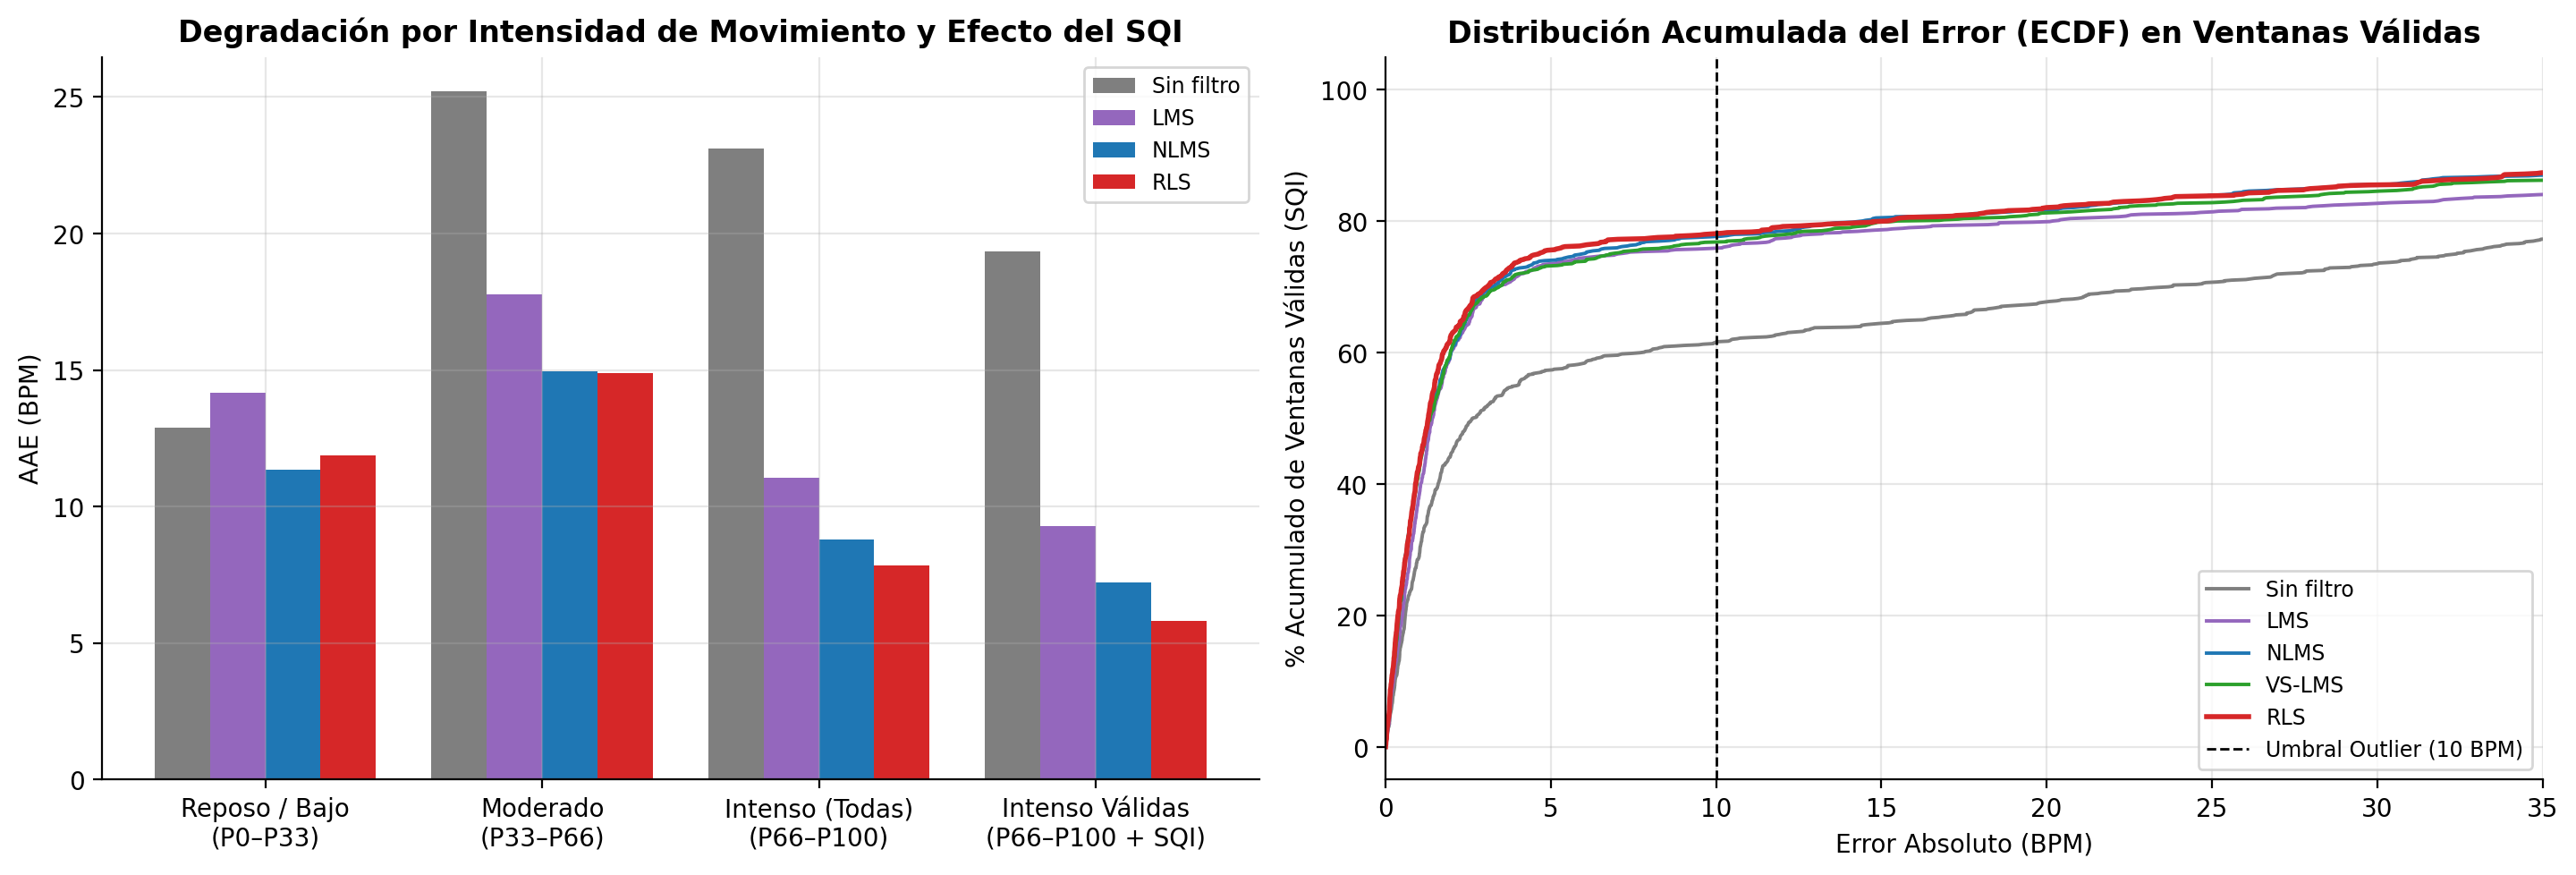
\includegraphics[width=0.55\textwidth]{Figures/05_regimenes_movimiento_y_ecdf.png}
    \caption{Izquierda: AAE por tercil de $E_{\text{ACC}}$ e impacto del SQI en movimiento intenso. Derecha: ECDF del error absoluto sobre las $1078$ ventanas válidas (esta imagen fue creada utilizando nuestro código).}
    \label{fig:regimen}
\end{figure*}

\begin{table}[!t]
    \centering
    \caption{Impacto del SQI ($P_{75}/P_{25}$, cobertura $81.2\%$) sobre el AAE en prueba (BPM). $p$: fracción de $1000$ descartes aleatorios con AAE igual o menor.}
    \label{tab:sqi}
    \footnotesize
    \setlength{\tabcolsep}{3pt}
    \begin{tabular}{lcccc}
        \toprule
        \textbf{Método} & \textbf{Global} & \textbf{Retenidas} & \textbf{Descartadas} & $p$ \\
        \midrule
        Sin filtro & $20.41$ & $19.11$ & $25.99$ & --- \\
        LMS & $14.35$ & $14.79$ & $12.43$ & $0.868$ \\
        NLMS & $11.71$ & $12.11$ & $9.99$ & $0.890$ \\
        VS-LMS & $12.23$ & $12.72$ & $10.09$ & $0.949$ \\
        RLS & $11.54$ & $12.03$ & $9.42$ & $0.933$ \\
        \bottomrule
    \end{tabular}
\end{table}

La Fig.~\ref{fig:regimen} (izquierda) explica esta paradoja por terciles de $E_{\text{ACC}}$: en reposo ($P_0$--$P_{33}$) NLMS ($11.37$) y RLS ($11.87$) apenas mejoran la base ($12.89\text{ BPM}$); con movimiento moderado ($P_{33}$--$P_{66}$) bajan el error de $25.21$ a $14.88$ (RLS) y $14.96\text{ BPM}$ (NLMS); y con movimiento intenso ($P_{66}$--$P_{100}$) RLS ($7.85$) y NLMS reoptimizado ($8.79\text{ BPM}$) logran la mayor ganancia frente a LMS ($11.07$) y la base ($23.10\text{ BPM}$). Dentro de ese tercil intenso, el SQI sí reduce el error de RLS de $7.85$ a $5.81\text{ BPM}$; sin embargo, al descartar ventanas de alta agitación en sujetos donde los filtros funcionan bien y dejar intactas las fallas de baja aceleración en los Sujetos~1, 2 y~7, sube la proporción de estos últimos y aumenta el AAE global (paradoja de Simpson). La ECDF sobre ventanas válidas (Fig.~\ref{fig:regimen}, derecha) confirma el desempeño muy parejo de RLS y NLMS.

\FloatBarrier
%==========================================================
\section{\secUC{Conclusiones}}
\label{sec:conc}
%==========================================================

En síntesis, al reoptimizar RLS, NLMS y VS-LMS sobre el mismo \textit{pipeline} y rango $M\in[6,50]$, la evaluación sobre el conjunto de prueba de IEEEPPG arroja cuatro conclusiones:
\begin{enumerate}
    \item \textbf{Rendimiento y significancia en prueba:} RLS logra el menor AAE ($11.54\text{ BPM}$), menor mediana ($1.30\text{ BPM}$, comparable a la literatura) y menos \textit{outliers} ($21.39\%$); supera significativamente a no filtrar ($+8.81\text{ BPM}$) y LMS ($+2.80\text{ BPM}$), pero frente a NLMS ($11.71\text{ BPM}$, RMSE $26.22$ vs.\ $26.23\text{ BPM}$) y VS-LMS ($12.23\text{ BPM}$) la brecha ($0.17$--$0.69\text{ BPM}$) no es concluyente con $10$ sujetos.
    \item \textbf{Modos, convergencia y costo:} sin precalentamiento, RLS converge en el límite teórico $2L/f_s=0.38\text{ s}$ ($-5.68\text{ dB}$, $\mathcal{M}_{\text{RLS}}=0.64\%$) evitando las constantes lentas ($\tau_5=10\text{ s}$) del LMS; con precalentamiento ($\text{WS}=0.25$) parte en $\approx -8.5\text{ dB}$ y cuesta $18.6\text{ ms}$ por ventana ($1.3\times$ NLMS compartiendo $\mathbf{P}(n)$), viable en tiempo real ($<1\%$ del paso de $2\text{ s}$).
    \item \textbf{Sensibilidad, estabilidad y dilatación:} en prueba el RLS ingenuo rinde peor que no filtrar ($23.83\text{ BPM}$) con explosión de pesos ($\lVert\mathbf{w}\rVert_2=3.54\times 10^4$); la regularización $\delta_0=\delta L$ acorde a $\hat{\mathbf{R}}$ ($2.5\%$ de $\lambda_{\max}$) con memoria larga ($N_{\text{eff}}=1881.4$, mejor que $\lambda=1$ y que $N_{\text{eff}}=150$) estabiliza $\lVert\mathbf{w}\rVert_2=0.382$. La dilatación ($D=3$) no es indispensable una vez activas $\delta_0$ y la carga diagonal, pero aporta condicionamiento y compresión $\mathcal{O}(L^2)$.
    \item \textbf{Límites físicos y SQI:} los peores errores (Sujetos~1, 2, 4 y~7) son comunes por distorsiones no lineales y saltos espectrales sin seguimiento entre ventanas. El SQI dual mejoró el tercil intenso ($7.85\to 5.81\text{ BPM}$), pero no superó al azar globalmente ($p=0.87$--$0.95$).
\end{enumerate}

Como trabajo futuro, convendría evaluar conjuntos con más participantes, agregar seguimiento temporal entre ventanas (p.\ ej.\ filtros de Kalman o programación dinámica~\cite{zhang2015troika}) para evitar saltos espectrales, diseñar SQI post-filtrado o morfológicos~\cite{elgendi2016sqi} sensibles a mal contacto en reposo, y explorar canceladores adaptativos no lineales frente a impactos impulsivos.

\bibliographystyle{IEEEtran}
\bibliography{references}

\end{document}
